\documentclass[12pt]{article}
\usepackage{authblk}
\usepackage[english]{babel}
\usepackage{threeparttable}
% Bibliography Style
\usepackage[authoryear]{natbib}  % Enables Chicago author-date citations
\bibliographystyle{chicago}

\usepackage{soul}
\usepackage{amsmath}
\usepackage{graphicx}   % Required for \resizebox{}
\usepackage[colorlinks=true, allcolors=blue]{hyperref}
 \newcommand\citeapos[1]{\citeauthor{#1}'s (\citeyear{#1})} % use apostrofe for references e.g. Lehr's (1990)
\makeatletter
 \def\@mb@citenamelist{cite,citep,citet,citealp,citealt,citeapos} % this will add the custom made command 'citeapos' to the list of newcite commands
 \makeatother
% Margins: 1-inch all around
\usepackage[margin=1in]{geometry}

% Font: Times New Roman (or closest equivalent)
% \usepackage{times}  

% Table & Formatting Packages
\usepackage{threeparttable} % For notes below tables
\usepackage{array}          % Improved column alignment
\usepackage{siunitx}        % Proper numeric alignment
\usepackage{booktabs}       % Professional table formatting
\usepackage{float}          % Ensures float placement control

% Caption Formatting
\usepackage{caption}   
\captionsetup[table]{
  labelsep = period, % "Table 1."
  justification = centering,
  font = bf, % Bold table caption
  textfont = {bf}
}

% Double spacing for the manuscript
\usepackage{setspace}
% \doublespacing

% Section Formatting
% \usepackage{titlesec}   
% \titleformat{\section}
%   {\large\bfseries}  % Large and bold
%   {\thesection\ \textbar}  % Section number followed by a vertical bar "|"
%   {0.5em}            % Space between "|" and title
%   {\MakeUppercase}   % Convert title to uppercase

\usepackage{xcolor}




\title{\textbf{Game structure obviousness in homegrown preference elicitation}}

\author[1]{Levenson Badio\thanks{Insert your info here.}}
\author[1]{Marco A. Palma\thanks{Professor and Director Human Behavior Laboratory, Department of Agricultural Economics, Texas A\&M University, College Station, TX  77843 USA, tel:+1-9798455284 e-mail: \href{mailto:mapalma@tamu.edu}{mapalma@tamu.edu}.}}
\author[2]{Andreas C. Drichoutis\thanks{Professor, Department of Agricultural Economics \& Rural Development, School of Applied Economics and Social Sciences, Agricultural University of Athens, Iera Odos 75, 11855, Greece, e-mail: \href{mailto:adrihout@aua.gr}{adrihout@aua.gr}.}}
\author[1]{Samuel Zapata\thanks{Insert your info here.}}
\author[1]{Rodolfo M. Nayga, Jr.\thanks{Professor and Head, Department of Agricultural Economics, Texas A\&M University, College Station, TX  77843 USA, and Adjunct Professor, Korea University; tel:+1-9798452116 e-mail: \href{mailto:rnayga@tamu.edu}{rnayga@tamu.edu}.}}

\affil[1]{Texas A\&M University}
\affil[2]{Agricultural University of Athens} 
\date{}

\begin{document}
\maketitle

\onehalfspacing
\begin{abstract}
\noindent The Becker-Degroot-Marschak (BDM) mechanism is widely used in experimental valuation research because of its theoretical incentive compatibility and implementation simplicity. However, recent work challenges BDM's ability to produce outcomes that closely represent its theoretical predictions in induced value (IV) settings. A relatively new method, the Game Structure Obvious (GSO) mechanism, has shown promising results in aligning IV theoretical predictions with empirical findings. The GSO mechanism however has not been tested in homegrown settings, which are particularly important in market research aimed at understanding demand for untested or unfamiliar products. We compare the BDM and the GSO mechanisms in an online homegrown experiment---eliciting consumers' preference for antibiotic-treated oranges, and compare the valuation outcomes in real and hypothetical treatments. Our findings reveal a counterintuitive methodological insight: while GSO is perceived as simpler and more intuitive than BDM in all treatments, the hypothetical GSO induces significant hypothetical bias in early decision rounds, while the BDM does not. The valuations elicited in all other treatment are statistically indistinguishable. However, the GSO mechanism shows remarkable learning effects, with hypothetical bias diminishing fast over subsequent rounds. 

\textbf{Keywords:} Strategy-proof, BDM, GSO, hypothetical bias, citrus greening, oranges. 
	
\textbf{JEL codes:} C90, C91, D44, D80
 
 \textbf{AEA RCT Registry:} AEARCTR-0014656
 
 \end{abstract}


\onehalfspacing
\section{Introduction}
Obtaining accurate estimates of individual valuations for products and services is crucial in guiding policy recommendations and product development innovations. Experimental auctions, and auction like mechanisms, are prominently used tools in valuation studies \citep{lusk2007experimental,canavari2019run}. However, reliably recovering true preferences remains a persistent challenge, even in cases where the good in question has a simple, fixed, and objectively measurable value \citep{drichoutis2022game, cason_misconceptions_2014}. One commonly used method for eliciting preferences, especially in settings where direct interaction with participants is limited, is the Becker-DeGroot-Marschak (BDM) mechanism which is favored for its simplicity and theoretical incentive compatibility \citep{mamadehussene2023reliability, azrieli2018incentives}. In the BDM mechanism, participants are asked to submit a bid for a good with the knowledge that a price is randomly drawn from a predetermined range. If the participant's bid is equal to or higher than the drawn price, they purchase the item at that price. Otherwise, they do not receive the item \citep{becker_measuring_1964}. Yet, evidence shows that participants often fail to bid their true valuation, even for goods with known and objective values, raising concerns about its behavioral incentive compatibility. Beyond its theoretical appeal, the BDM mechanism is also widely used in online studies to measure valuations, beliefs, subjective probabilities, and trust  \citep{mamadehussene2023reliability, holt2009update, karni2009mechanism,shikuku2023endowments}. 

Despite its notable limitations and the fact that it under-performs auction mechanisms like the second price auction \citep{DrichoutisEtAl2024incentives}, the BDM mechanism continues to be widely used in value elicitation experiments. \citet{cason_misconceptions_2014} highlighted pitfalls of the BDM mechanism within an induced value framework, where participants were asked to provide their willingness to accept (WTA) for a card with a fixed value of \$2. Given that the value of money is objective and fixed, the experiment directly challenged the theoretical incentive compatibility of the BDM mechanism by showcasing that only 16.7\% of participants bid within 5\% of the actual value of \$2.\footnote{However, bidding accuracy (within the \$2) increases with learning and roughly doubles by the second round of bidding \cite{cason_misconceptions_2014}.} This issue is not unique to the BDM mechanism; \citet{DrichoutisEtAl2024incentives} report similar findings to \citet{cason_misconceptions_2014} with only 24.7\% of bidders submitting bids within 5\% of the induced value in the BDM mechanism, while second-price auctions show only modest improvements to 27.4\%. Given this failure to bid within the expected objective value of money in such a simple induce value setting, it is reasonable to question the validity of these commonly used mechanisms as accurate market preference elicitation tools. 

The persistent failure of existing elicitation mechanisms to consistently induce weakly dominant strategies in induced value settings has motivated the development of new strategy-proof methods designed to make optimal choices more apparent to participants \citep{li_obviously_2017, pycia_theory_2023}. Strategy proof mechanisms simply mean that respondents reveal their preferences truthfully, and deviating from it produces no gains. Among these, the Game Structure Obvious (GSO) mechanism has emerged as a novel and increasingly prominent tool. It is recognized for being strategy-proof and for making weakly dominant strategies obvious to participants. 

In the context of homegrown valuation, the GSO mechanism operates as a multiple price list in which participants choose, at each step, whether to purchase or decline an item at a given price \citep{yu2021multiple, herberich2012digging, jack2022multiple}.  The price starts at a fixed level and increases by a constant amount until it reaches a terminal value randomly determined at the outset. We argue that it is important to compare the GSO with the BDM mechanism in a homegrown setting for two reasons. For one, in induced value settings, the GSO mechanism has achieved significantly higher rates of bids consistent with theoretical predictions (between 43\% and 58\%) than other elicitation mechanisms but we are unaware if this finding transfers verbatim to a homegrown setting. Secondly, since the GSO mechanism has not yet been empirically applied in homegrown valuation studies, its reliability in settings involving hypothetical scenarios remains an open question. In homegrown valuation studies, the value of the object is not objectively determined, hence we focus on which elicitation method elicits valuations further away from hypothetical values.  This topic is important to address given that market and resource valuations are more complex and often involve the evaluation of multiple attributes and information.  Thus, it is critical to evaluate the performance of the GSO and BDM mechanisms under both hypothetical and incentivized conditions to establish meaningful benchmarks for future use. 

We implemented an online experiment recruiting participants in the U.S in order to test the performance of the GSO and BDM mechanisms under real and hypothetical incentives; the hypothetical treatments served as our benchmark. As a case study, we elicited consumers' willingness to pay (WTP) for orange fruits from trees treated with trunk-injected antibiotics for Huanglongbing (HLB) and conventionally grown oranges.
% This is too much information for the intro: Each participant received a \$6 endowment (except in hypothetical treatments, in which case participants were informed that decisions were not binding but encouraged to respond as if they were real). Elicitation tasks occurred over three rounds. Participants bid simultaneously on two types of oranges.

Our results point to a few stylized facts. For one, subjects in our experiment find the GSO mechanism less complex than the BDM, consistent with it being more game strategy obvious. Paradoxically though, while we find no evidence of hypothetical bias in the BDM mechanism, we find clear evidence of hypothetical bias in the GSO mechanism. When disaggregating the analysis by round, our results suggest that there is however, significant learning in the GSO mechanism such that hypothetical bias reduces over subsequent rounds. In contrast, there is no evidence of learning in the BDM mechanism.
Moreover, we find that under real incentives, WTP elicited with the BDM and the GSO mechanism are statistically indistinguishable. However, under hypothetical incentives, the GSO mechanism consistently produces significantly higher WTP values than the BDM mechanism.

Our findings provide a critical methodological contribution in preference elicitation research. Contrary to expectations based on induced value settings, the study reveals a nuanced and counterintuitive insight: while the GSO mechanism demonstrates lower perceived complexity, it fails to mitigate hypothetical bias. This challenges the common assumption that simpler and more transparent mechanisms inherently yield more accurate preference estimates. At the same time, it highlights that results from induced value settings do not transfer verbatim to homegrown settings, where preferences are subjective and context-dependent. The GSO mechanism, however, remains superior in promoting learning, as it appears to help participants more easily recognize their best-response strategies over time.

We contribute to the literature in two ways. First, our study relates to the literature on strategy-proof mechanisms in preference elicitation, particularly those that aim to make the weakly dominant strategy obvious \citep{li_obviously_2017, pycia_theory_2023, chakraborty_future_2025}. While previous research has demonstrated GSO's superiority in induced value settings, where participants bid on items with known and objective values,  our study is the first to systematically test GSO's effectiveness in a homegrown valuation context where true values are subjective and unknown. We challenge the implicit assumption that mechanisms performing well in induced value settings will automatically translate to superior performance in a real consumer valuation context. Second, our study contributes to the hypothetical bias literature \citep{penn2018understanding, cummings1999unbiased, loomis_whats_2011, fang_use_2021, list2001explicit, grebitus2013explaining}; we find evidence of hypothetical bias in the simpler GSO mechanism but no hypothetical bias in the more complex BDM mechanism. Therefore, our counterintuitive finding challenges conventional wisdom about the relationship between mechanism simplicity and bias mitigation. Finally, our study contributes to applied consumer research by demonstrating how methodological choices in preference elicitation can substantially affect elicited valuations and should not be naively or by default applied in valuation studies \citep{miller2011should, schmidt2020accurately}.

\hl{Our paper proceeds as follows. In the next section we describe our experimental design, procedures and data collection \ldots}

\section{Experimental methods}
In the next subsections we describe... (give a short overview of what's coming...)

\subsection{Experimental Design}
Our study employed a $2\times2$ between-subjects design that varied across two dimensions: elicitation method (BDM vs. GSO mechanism) and incentives (Hypothetical vs. Real incentives). Subjects were randomly assigned to one of the four treatment groups. In the hypothetical incentives treatment, subjects were told that none of the described payoffs or potential purchases were real or were actually going to take place and they would only receive a participation fee. In the real incentives treatment, we implemented a Between-subjects Random Incentivized Scheme (BRIS) with a 10\% realization probability \citep{ahles_testing_2024}. On top to their participation fee, each participant was endowed with \$6 that they could potentially use to buy a pound of oranges during the experiment with the understanding that any money they did not use would be added to their bonus payment. Subjects submitted bids in three consecutive rounds and at each round they could bid for a pound of conventional oranges and a pound of oranges from trees treated with antibiotics. Subjects were told that at the end of the experiment one round and one product would be randomly drawn as binding and any transactions regarding that product and round would be realized. 

% \footnote{ However, for the hypothetical treatments, participants were explicitly informed of the hypothetical nature of the endowment and decisions.}  

The elicitation task was conducted in three rounds to account for learning \citep{corrigan2008testing, drichoutis2011role} in value elicitation. The first two rounds of bidding were exactly the same (i.e., no new information was added between the rounds) and with only basic information about the types of oranges. Before the third round, we introduced an information treatment video that informed subjects about the impact of HLB on the US citrus industry.\footnote{Participants watched a 51 seconds video containing objective information about the impact of HLB on the US citrus industry, the livelihood of farmers, and its potential risk to human health and the environment. The information script was revised by agricultural scientists to ensure veracity and accuracy of the information. This design allows us to measure the impact of information provision on WTP for oranges from antibiotic-treated orange trees relative to conventional oranges.}  In both the BDM and the GSO mechanism treatments, the randomly determined prices were randomly drawn from a uniform distribution of [\$0, \$6] with increment of \$0.20.\footnote{The upper bound of the range was chosen based on the actual maximum value of the orange prices in the market at the time of the study plus a price premium of 40\% higher than the market price for those willing to pay a premium for oranges from antibiotic-treated orange trees.}

In the BDM mechanism treatment, subjects had to use a slider to select their bid. If their bid for one pound of oranges was greater than or equal to the randomly drawn price, they would buy the product at the randomly drawn price, otherwise, they would not buy the product and would keep their endowment. 
% \citet{masuda_net_2022} found that in a Vickrey auctions for an an item \footnote{The item was not a real product. It was described in a neutral term, it can be thought as an induced values setting.}, when participant learns about the incentive compatibility, it increases their likelihood to bid their true valuation by 47\% compared to subjects who did not receive the advice. 

% The GSO mechanism functions similarly to an ascending clock auction. In the experiment, participants made purchasing decisions across two randomized market settings: one for conventional oranges and another for antibiotics- oranges. In each market, they had two options: .

At the start of each round, an `Offer Price' appeared on the screen that was subsequently increased in fixed increments of \$0.20 after each decision they made. The offer price for the first screen was set to \$0. The process of increasing the offer price was continued until it reached a randomly drawn `market price', which was unknown to participants. The random price was independently drawn for each round from a uniform distribution between \$0 and \$6 and was different between subjects, rounds and treatments. When the offer price matched the randomly drawn price, the round automatically ended.\footnote{See Figure~\ref{fig:Appendix_GSO_game} in the Appendix for an illustration and a link to a video capture of how this dynamic process looked like.} For each price step, participants chose between two options labeled as ``Try to Buy'' or ``Do Not Buy''. If subjects selected ``Do Not Buy'' even at least once, they would not be allowed to buy if that round is selected (even if they switch back to buy). 

If participants always selected ``Try to Buy'' for an orange product, they had the possibility of purchasing the bag of oranges according to their treatment. However, if they selected ``Not Buy'' at least once, they would not be able to buy the product if that round and product were selected (even if they decide switch back to ``Try to Buy'' at that round). 

One characteristic of the GSO mechanism is that it does not prevent multiple switching. Specifically, individuals who may initially decide not to purchase at a given (low) price may later attempt to buy at a higher price in subsequent rounds. To reduce multiple switching due to accidental clicking or lack of attention, we implemented a soft nudge consisting of a warning to multiple switchers, reminding them of the last price they chose not to buy, with the option of changing their inconsistent choice \citep{yu2021multiple}.\footnote{Participants retained full freedom to make choices as they wished. To address potential input errors (e.g., trembling hands or accidental clicks), a confirmation prompt was displayed whenever a participant switched from opting to buy to not buying: ``You are deciding not to buy at this price. Do you want to confirm it?''} %\footnote{However, participants had the freedom to choose as s/he desires. Also, since trembling hands can be an issue in the experiment, When participants switch from trying to buy to not buy, We provide a notification (You are deciding not to buy at this price. Do you want to confirm it?)} 
This intervention was designed to reduce the multiple switching behavior caused by inattention. Our main analysis does not exclude multiple switchers from the GSO treatment, as these participants may genuinely prefer randomization \hl{(cite: https://www.journals.uchicago.edu/doi/abs/10.1086/689774 and https://www.aeaweb.org/articles?id=10.1257/pandp.20221093)}. %In addition, including them helps avoid selection bias when comparing GSO with BDM, where similar behavior might also occur. For completeness, we report results excluding multiple switchers in the appendix.
    
\subsection{Experimental Procedures}
The experiment was programmed in Qualtrics and the study protocol was approved by the Institutional Review Board (IRB) at Texas A\&M University in October 2024 (approval number...). Our study was pre-registered with the AEA's RCT registry (\href{https://www.socialscienceregistry.org/trials/14656}{AEARCTR-0014656
}). A total of 1,237 U.S. general population participants were recruited through Forthright Access, an online research company that handles their own recruitment through a variety of direct advertising channels. The data were collected in December 2024. To be eligible, participants had to be at least 18 years old and purchase and eat citrus at least once a month. 
Each participant received a base participation fee of \$2 for completing the study. The study started with participants receiving treatment-specific instructions, followed by comprehension questions. In the real incentivized treatment, participants were informed that they would complete three rounds of elicitation tasks and that one product from a randomly chosen round would be randomly chosen for realization. %Randomly choosing one round for payment has been shown to preserve the incentive compatibility of the mechanism, ensuring that participants give equal importance to each decision \citep{azrieli2018incentives}. 

After completing the main bidding task, participants responded to a post-experiment survey to measure perceived complexity using the simplified and validated measure of \citet{enke_cognitive_2023},  choice certainty. For the real incentivized treatments, a random number determined the realization with 10\% probability.  If selected, the winner would receive any remaining funds from their endowment and was asked to voluntarily provide a shipping address to deliver (free of charge) the oranges via priority mail. A separate link was provided to enter the mailing address information to preserve anonymity. A total of 108 (8.7\%) participants were selected for payment, and we shipped oranges to 45 subjects. The rest were non-buyers who just received their endowment of \$6 on top of their participation fee. 
%Among the 45 buyers, 36 provided a mailing address and were subsequently shipped the oranges; they also received any remaining balance from their endowment.

% \subsection{Data}
A total of 1,926 participants initially started the study. Of these, 689 subjects failed to meet the screening criteria, did not pass attention checks, or did not complete the study. This resulted in a final sample of 1,237 participants with complete responses. 

%Among this sample, 14.31\%, 9.60\%, and 3.87\% of participants in rounds 1, 2, and 3, respectively, were classified as multiple switchers (MS). Following the approach of \citet{brown2018separated}, we included these participants in the main analysis, interpreting MS behavior as a potential indication of a preference for randomization within an indifference range \citep{agranov2023stable}. This process also allows for comparability with the BDM mechanism.  As a robustness check, we also report results excluding multiple switchers; our findings remain broadly consistent. 


\section{Econometric analysis}
To analyze our data we use random effects interval regression models to account for the nature of the interval data elicited with the GSO mechanism as well as the panel nature of the data. Unlike standard valuation methods, the GSO mechanism captures WTP within an interval, rather than a single value. Specifically, a participant's valuation is bounded between the switch point between `Try to Buy' and `Do Not Buy'. The model can also accommodate point valuations elicited with the BDM mechanism. In our data, 1.5\% of observations is left censored at \$0, while 3\% is right censored at \$6. Since we collected repeated measurements, we also incorporated fixed effects to control for unobserved individual heterogeneity. \hl{If these are the demographics then write so...} To improve inference under potential heteroskedasticity, we applied 1,000 bootstrap iterations to estimate robust standard errors.

To compare elicited valuations between the treatments, we use the following specification:
\vspace{-1cm}

\begin{equation}\label{eq:specification}
Y_{it}^* = \gamma_0 + \gamma_1 \cdot \text{GSO}_i + \gamma_2 \cdot \text{Hypo}_i + \gamma_3 \cdot \text{(GSO} \times \text{Hypo)}_i + \alpha_i + \varepsilon_{it} 
\quad \varepsilon_{it} \sim \mathcal{N}(0, \sigma^2)
\end{equation}


% \noindent
In this specification, $Y_{it}^*$ denotes the latent WTP for individual $i$ at round $t$, with $t = 1, 2, 3$. For the BDM mechanism treatment groups, it is  $Y_{it}^*$= $Y_{it}$; for the GSO mechanism, WTP comes in intervals defined by subjects' switching point. \hl{the following explanation should be moved in the appendix, but first remove the bullet points}:
% \begin{itemize}
%     \item $Y_{it}^* \in [\text{Try to Buy}, 6]$ if the computer accepted the price in the GSO treatment group;
%     \item $Y_{it}^* \in [\text{Try to Buy}, \text{Not Buy})$ if the participant switched to "Not Buy" during the elicitation
%     \item $Y_{it}^* \in [\text{Not Buy}^-; \text{Not Buy}^+]$, in which $\text{Not Buy}^-$, and $\text{Not Buy}^+$ represent the first and the last time participants click this option, respectively. \footnote{ This is in the case of multiple switching following \citet{brown2018separated}.}
% \end{itemize}

% \noindent
In Equation~\ref{eq:specification}, $\text{GSO}_i$ is a dummy variable indicating assignment to the GSO mechanism treatment and $\text{Hypo}_i$ is a dummy variable indicating assignment to the Hypothetical incentives treatment. The specification also includes their interaction, $\text{GSO}_i \times \text{Hypo}_i$, while $\alpha_i$ captures individual-specific fixed effects and $\varepsilon_{it} \sim \mathcal{N}(0, \sigma^2)$ is an idiosyncratic error term for individual $i$ at round $t$.
    % \item $\text{GSO}_i \times \text{Hypo}_i$ is an interaction term equal to 1 if individual $i$ is in the GSO Hypothetical treatment group;
    % \item$ \gamma_0$: Baseline (BDM Real)
    % \item $ \gamma_1, \gamma_2, \gamma_3$ represent mean differences in WTP relative to the BDM Real group (baseline category);
    
    % \item $\varepsilon_{it} \sim \mathcal{N}(0, \sigma^2)$ is an idiosyncratic error term for individual $i$ at round $t$.

Alternative specifications to Equation~\ref{eq:specification}, control for rounds (third round also coincides with information provision), type of orange and multiple switching behavior.

% In model 2 (see below), we control for the rounds effect and the type of oranges given that not only we have more than one round,but we also introduced information specicific to orange types. We also control for other variables such as risk preferences and demographic variables in model 3.
% \vspace{-1cm}

% \begin{multline}
% Y_{it}^* = \gamma_0 + \gamma_1 \cdot \text{GSO}_i + \gamma_2 \cdot \text{Hypo}_i + \gamma_3 \cdot (\text{GSO}_i \times \text{Hypo}_i) + \gamma_4 \cdot  \text{Round}_i + \gamma_5 \cdot \text{MSB}_i +\\
%   \alpha_{i} + \varepsilon_{it} 
% \quad \varepsilon_{it} \sim \mathcal{N}(0, \sigma^2)
% \end{multline}

% \vspace{-2cm}

% \begin{multline}
% Y_{it}^* = \gamma_0 + \gamma_1 \cdot \text{GSO}_i + \gamma_2 \cdot \text{Hypo}_i + \gamma_3 \cdot (\text{GSO}_i \times \text{Hypo}_i) + \gamma_4 \cdot \text{Round}_i + \gamma_5 \cdot \text{MSB}_i + \\  \theta_1 \cdot \text{(X)}_i  + \alpha_i + \varepsilon_{it} 
% \quad \varepsilon_{it} \sim \mathcal{N}(0, \sigma^2)
% \end{multline}


% \begin{itemize}
%     \item \textit{MSB}$_i$ is a dummy variable equal to 1 if a participant is a multiple switcher.
    
%     \item \textit{X}$_i$ is a vector of individual-level control variables (e.g., risk preferences, demographics).
% \end{itemize}
% \section{Hypotheses}
% Our main research hypotheses focus on determining which elicitation method leads to the lowest hypothetical bias mitigation. \footnote{Finally, we expect that information about the severity of disease on the domestic production of citrus fruits will induce people to increase their support and premium for citrus from trees treated with AB since consumers tend to support local farming and products, and information will have  positive effect on WTP. We hypothesize that information about the severity of the disease will lead to a higher WTP for AB-treated citrus.}
% Given the obviousness of GSO, it will be easier to identify weakly dominant strategies as compared to BDM. Because players do not need to anticipate future contingencies \citep{chakraborty_future_2025}, subjects in the GSO are more likely to reveal WTP according to their true preferences \citep{chakraborty_future_2025}.

% H1: GSO will lead to lower perceived complexity as compared to BDM.

% H2: The hypothetical bias will be lower in the GSO as compared to the BDM.


\section{Results}
To check whether randomization worked as expected, We first calculated standardized differences across treatments \citep{CochranRubin1973}. We find that our sample is well balanced.\footnote{While many researchers use statistical tests to check for balance of observable characteristics between treatments, the literature points to some pitfalls of this practice \citep[e.g.,][]{canavari2019run,DeatonCartwright2016,BrizEtAl2017,HoEtAl2007,MoherEtAl2010,MutzPemantle2015}. Following this literature, we report in Table \ref{tab:Appendix_std_diff_table} in the Appendix standardized differences across treatments \citep{ImbensRubin2016,ImbensWooldridge2009}. \citeapos{CochranRubin1973} rule of thumb is that the standardized difference should be less than 0.25. }
\hl{Do we also have the demographics of the 1926 - 1237 = 689 subjects that started but did not finish the study or were excluded for any reason? It would be useful to compare the demographics between the sample that completed the study with the sample of subjects filtered out of the study. } % We report standardized differences of observables across the treatments to test whether we have successfully achieved randomization (  see Table \ref{tab:Appendix_std_diff_table} in appendix). 


Our main result is based on data that includes multiple switchers since this might reflect indecisiveness in preferences elicited with the GSO mechanism. As a robustness check, we also report results excluding multiple switchers. Doing so, does not affect our main findings.

\hl{I would remove the following table (put it in the appendix) and present the marginal effects of GSO real, GSO hypothetical, BDM real, BDM hypothetical in a four row table (along with CIs). Additional rows below the table would indicate whether the model includes control for MSB or demographics. See below what you need to report in this table using margins in Stata (numbers are based on model 1).}

\begin{figure}
    \centering
    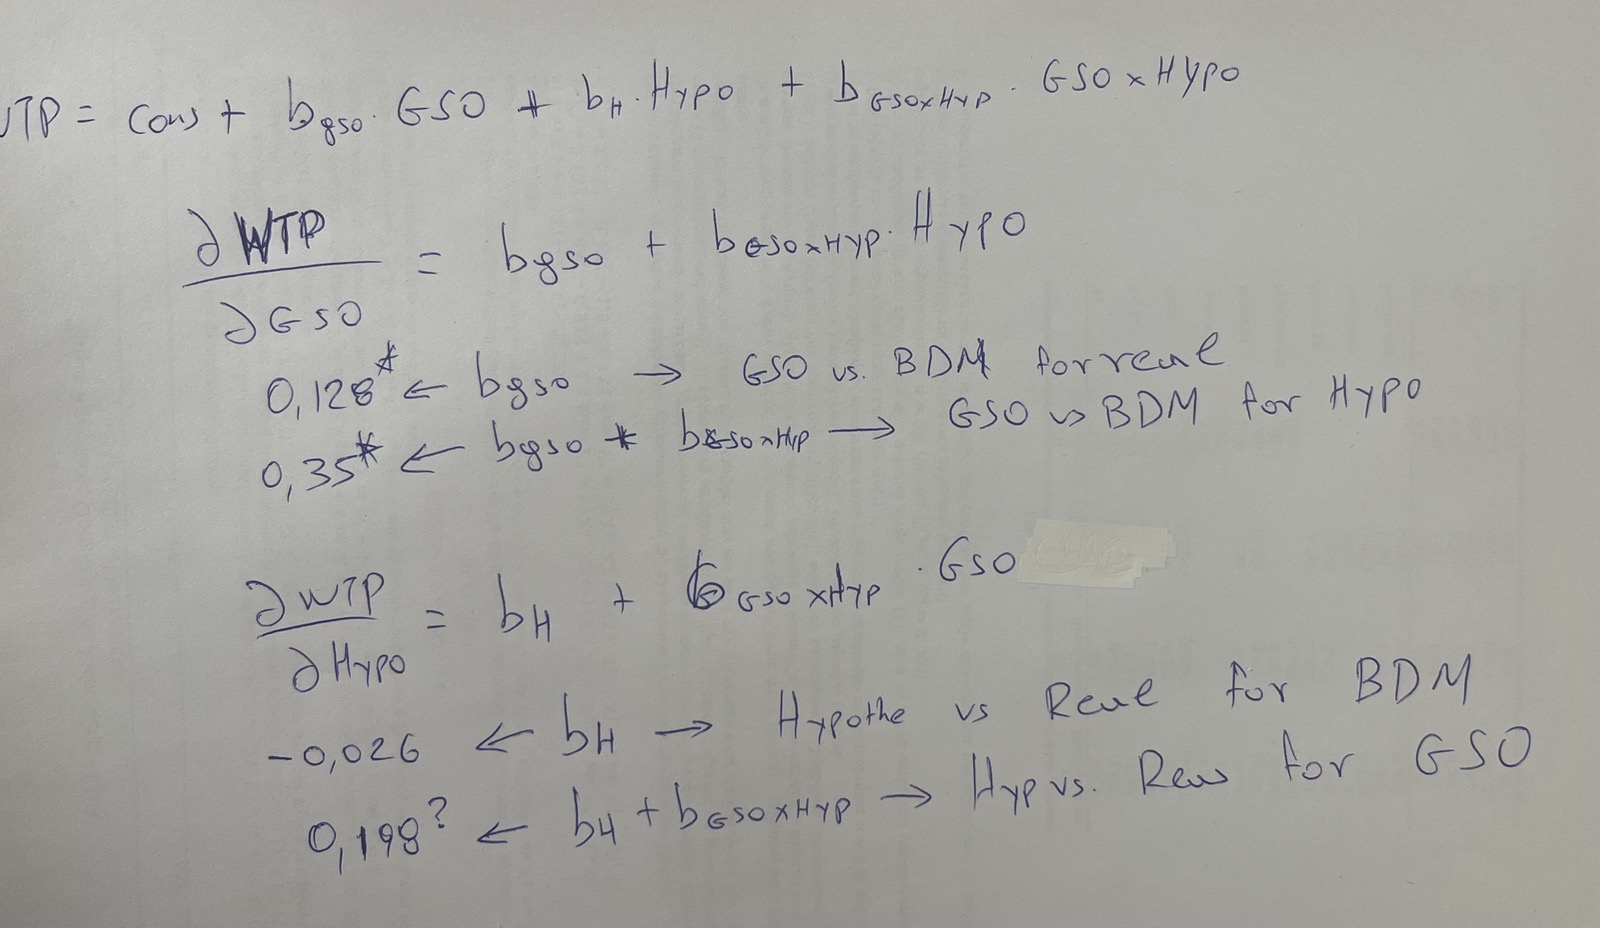
\includegraphics[width=0.7\linewidth]{wtp.jpg}
    \caption{Enter Caption}
    \label{fig:enter-label}
\end{figure}
 \begin{table}[H]
                \centering
                \caption{Interval Model of Consumer WTP for Oranges (Baseline: BDM Real)}
                \label{tab:interval_regression}
                \resizebox{0.8\textwidth}{!}{% Scale table to fit the column width
     \begin{tabular}{l*{3}{cc}}
\hline\hline
            &\multicolumn{2}{c}{(1)}           &\multicolumn{2}{c}{(2)}           &\multicolumn{2}{c}{(3)}           \\
            &\multicolumn{2}{c}{WTP}    &\multicolumn{2}{c}{WTP (control 1)}    &\multicolumn{2}{c}{WTP (control 2)}    \\
\hline
Constant    &       3.475\sym{***}&     (0.022)&       3.475\sym{***}&     (0.022)&       3.187\sym{***}&     (0.066)\\
GSO         &       0.128\sym{***}&     (0.040)&       0.048         &     (0.041)&       0.014         &     (0.040)\\
Hypothetical&      -0.026         &     (0.035)&      -0.027         &     (0.035)&      -0.037         &     (0.033)\\
GSO$\times$Hypothetical&       0.224\sym{***}&     (0.060)&       0.204\sym{***}&     (0.059)&       0.277\sym{***}&     (0.057)\\
MSB      &                     &            &       1.039\sym{***}&     (0.087)&       1.088\sym{***}&     (0.090)\\
Round2     &                     &            &                     &            &       0.060\sym{**} &     (0.029)\\
Round3     &                     &            &                     &            &       0.111\sym{***}&     (0.029)\\
Risk preferences&                     &            &                     &            &      -0.120\sym{***}&     (0.014)\\
White       &                     &            &                     &            &      -0.058\sym{**} &     (0.029)\\
Middle Income&                     &            &                     &            &      -0.045         &     (0.031)\\
High Income &                     &            &                     &            &       0.065         &     (0.048)\\
Midwest     &                     &            &                     &            &      -0.186\sym{***}&     (0.042)\\
South       &                     &            &                     &            &      -0.094\sym{**} &     (0.037)\\
West        &                     &            &                     &            &      -0.158\sym{***}&     (0.040)\\
Female      &                     &            &                     &            &       0.061\sym{**} &     (0.025)\\
Bachelor    &                     &            &                     &            &      -0.084\sym{***}&     (0.030)\\
No Children &                     &            &                     &            &       0.004         &     (0.030)\\
Married     &                     &            &                     &            &      -0.086\sym{***}&     (0.031)\\
Age         &                     &            &                     &            &       0.010\sym{***}&     (0.001)\\
$\sigma_u$     &       1.090\sym{***}&     (0.012)&       1.078\sym{***}&     (0.012)&       1.064\sym{***}&     (0.012)\\
$\sigma_e $    &       0.847\sym{***}&     (0.013)&       0.838\sym{***}&     (0.013)&       0.835\sym{***}&     (0.014)\\

\hline
\(n\) (observations)      &        7296         &            &        7296         &            &        7110         &            \\
\hline
\(N\) (subjects)      &        1216          &            &         1216          &            &        1185         &            \\
\hline\hline
\multicolumn{7}{l}{\footnotesize Standard errors in parentheses. * p$<$0.1, ** p$<$0.05 *** p$<$0.01}\\
\end{tabular}
}


\begin{tablenotes}
            \footnotesize
            \item Standard errors in parentheses. * p$<$0.1, ** p$<$0.05, *** p$<$0.01.
            \item \textit{Note:} $\sigma_u$ and $\sigma_e$ denote the standard deviations of the random intercept and residual error, respectively.\\
            $\times$: interaction\\
        \end{tablenotes}
            \end{table}



\textbf{Result 1:} There is no statistical difference between  the mean WTP in the real and the hypothetical BDM treatments. 

One of the main objectives of this research paper is to compare which method between BDM and GSO performs better in terms of hypothetical bias mitigation. Referring to table \ref{tab:interval_regression}, we can see the hypothetical bias value is close to zero and not statistically significant (\(\Delta = -0.037\), \(p > 0.1\)). This shows that the BDM performs does not have hypothetical bias. A graphical representation of this result is when in Figure \ref{fig:margin_hypo}.  This finding is in line with the growing literature on the use of incentives in experiments that support the idea that people can, in hypothetical settings, elicit valuations similar to those real settings \citep{branas-garza_paid_2023, drichoutis_incentives_2025}. \hl{Most other papers show hypothetical bias so not sure what is the right balance to show evidence against the majority of previous studies.}
\vspace{0.5cm}

\textbf{Result 2:} GSO hypothetical provides mean valuation statistically higher than GSO real. 

Turning our attention to GSO, our results provide clear evidence of hypothetical bias: valuations in the hypothetical setting are statistically higher than those in the non-hypothetical setting (\(\Delta = 0.24\), \(p < 0.001\)), this represents  an increase of a 7.5\% (see column 3 in the regression Table \ref{tab:interval_regression}). This finding aligns with previous literature suggesting that individuals tend to overstate their valuations in hypothetical scenarios compared to real financial settings \citep{penn2018understanding, fang_use_2021}. Figure \ref{fig:margin_hypo} graphically illustrates this difference, showing that GSO valuations under the hypothetical setting are significantly higher at the 95\% confidence level. 

This result is particularly noteworthy—and somewhat surprising—because we observe hypothetical bias in the GSO mechanism but not in the BDM. This is unexpected, as GSO is generally considered more game-transparent than BDM and is often thought to elicit valuations that more closely reflect the induced value. We explore possible explanations for this outcome in Section 5.3.
\vspace{0.5cm}



\textbf{Result 3:} Under real financial incentives, GSO and BDM produce statistically different estimates in the regression model. 
One thing to notice in Table \ref{tab:interval_regression} is that not controlling for MSB, under real incentives, GSO and BDM valuations differ, however controlling for MSB, they produce statistically equivalent.
When comparing BDM and GSO across conditions, we first observe that under real financial incentives, the two elicitation methods produce statistically different valuations, with BDM yielding significantly higher values than GSO (\(\Delta = 0.014\), \(p > 0.10\)). The model-based predicted values also supports this finding as shown in figure \ref{fig:margin_hypo}.
\vspace{0.5cm}

\textbf{Result 4:} Under hypothetical scenario, GSO produces valuation that are statistically higher than BDM.

One thing to notice from figure \ref{fig:margin_hypo}, is that GSO provides stastically higher valuation also in magnitude as compared to the other treatments. This supports the results previously discussed. Specifically, when comparing valuations in the hypothetical setting, we find significantly higher values under GSO compared to BDM  (\(\Delta = 0.277\), \(p = 0.000\)). GSO  is 8.7\% higher as compared to BDM in hypothetical setting. Given that we previously detected hypothetical bias in GSO but not in BDM, this raises concerns about the reliability of GSO-based valuations under hypothetical conditions. Based on these findings, BDM appears to be a more reliable elicitation method than GSO for hypothetical experimental settings.




\hl{use a different sceme for Figure 2 so that x-axis extends across the full axis .Also, start y-axis from zero.}

\begin{figure}[H]
    \centering
    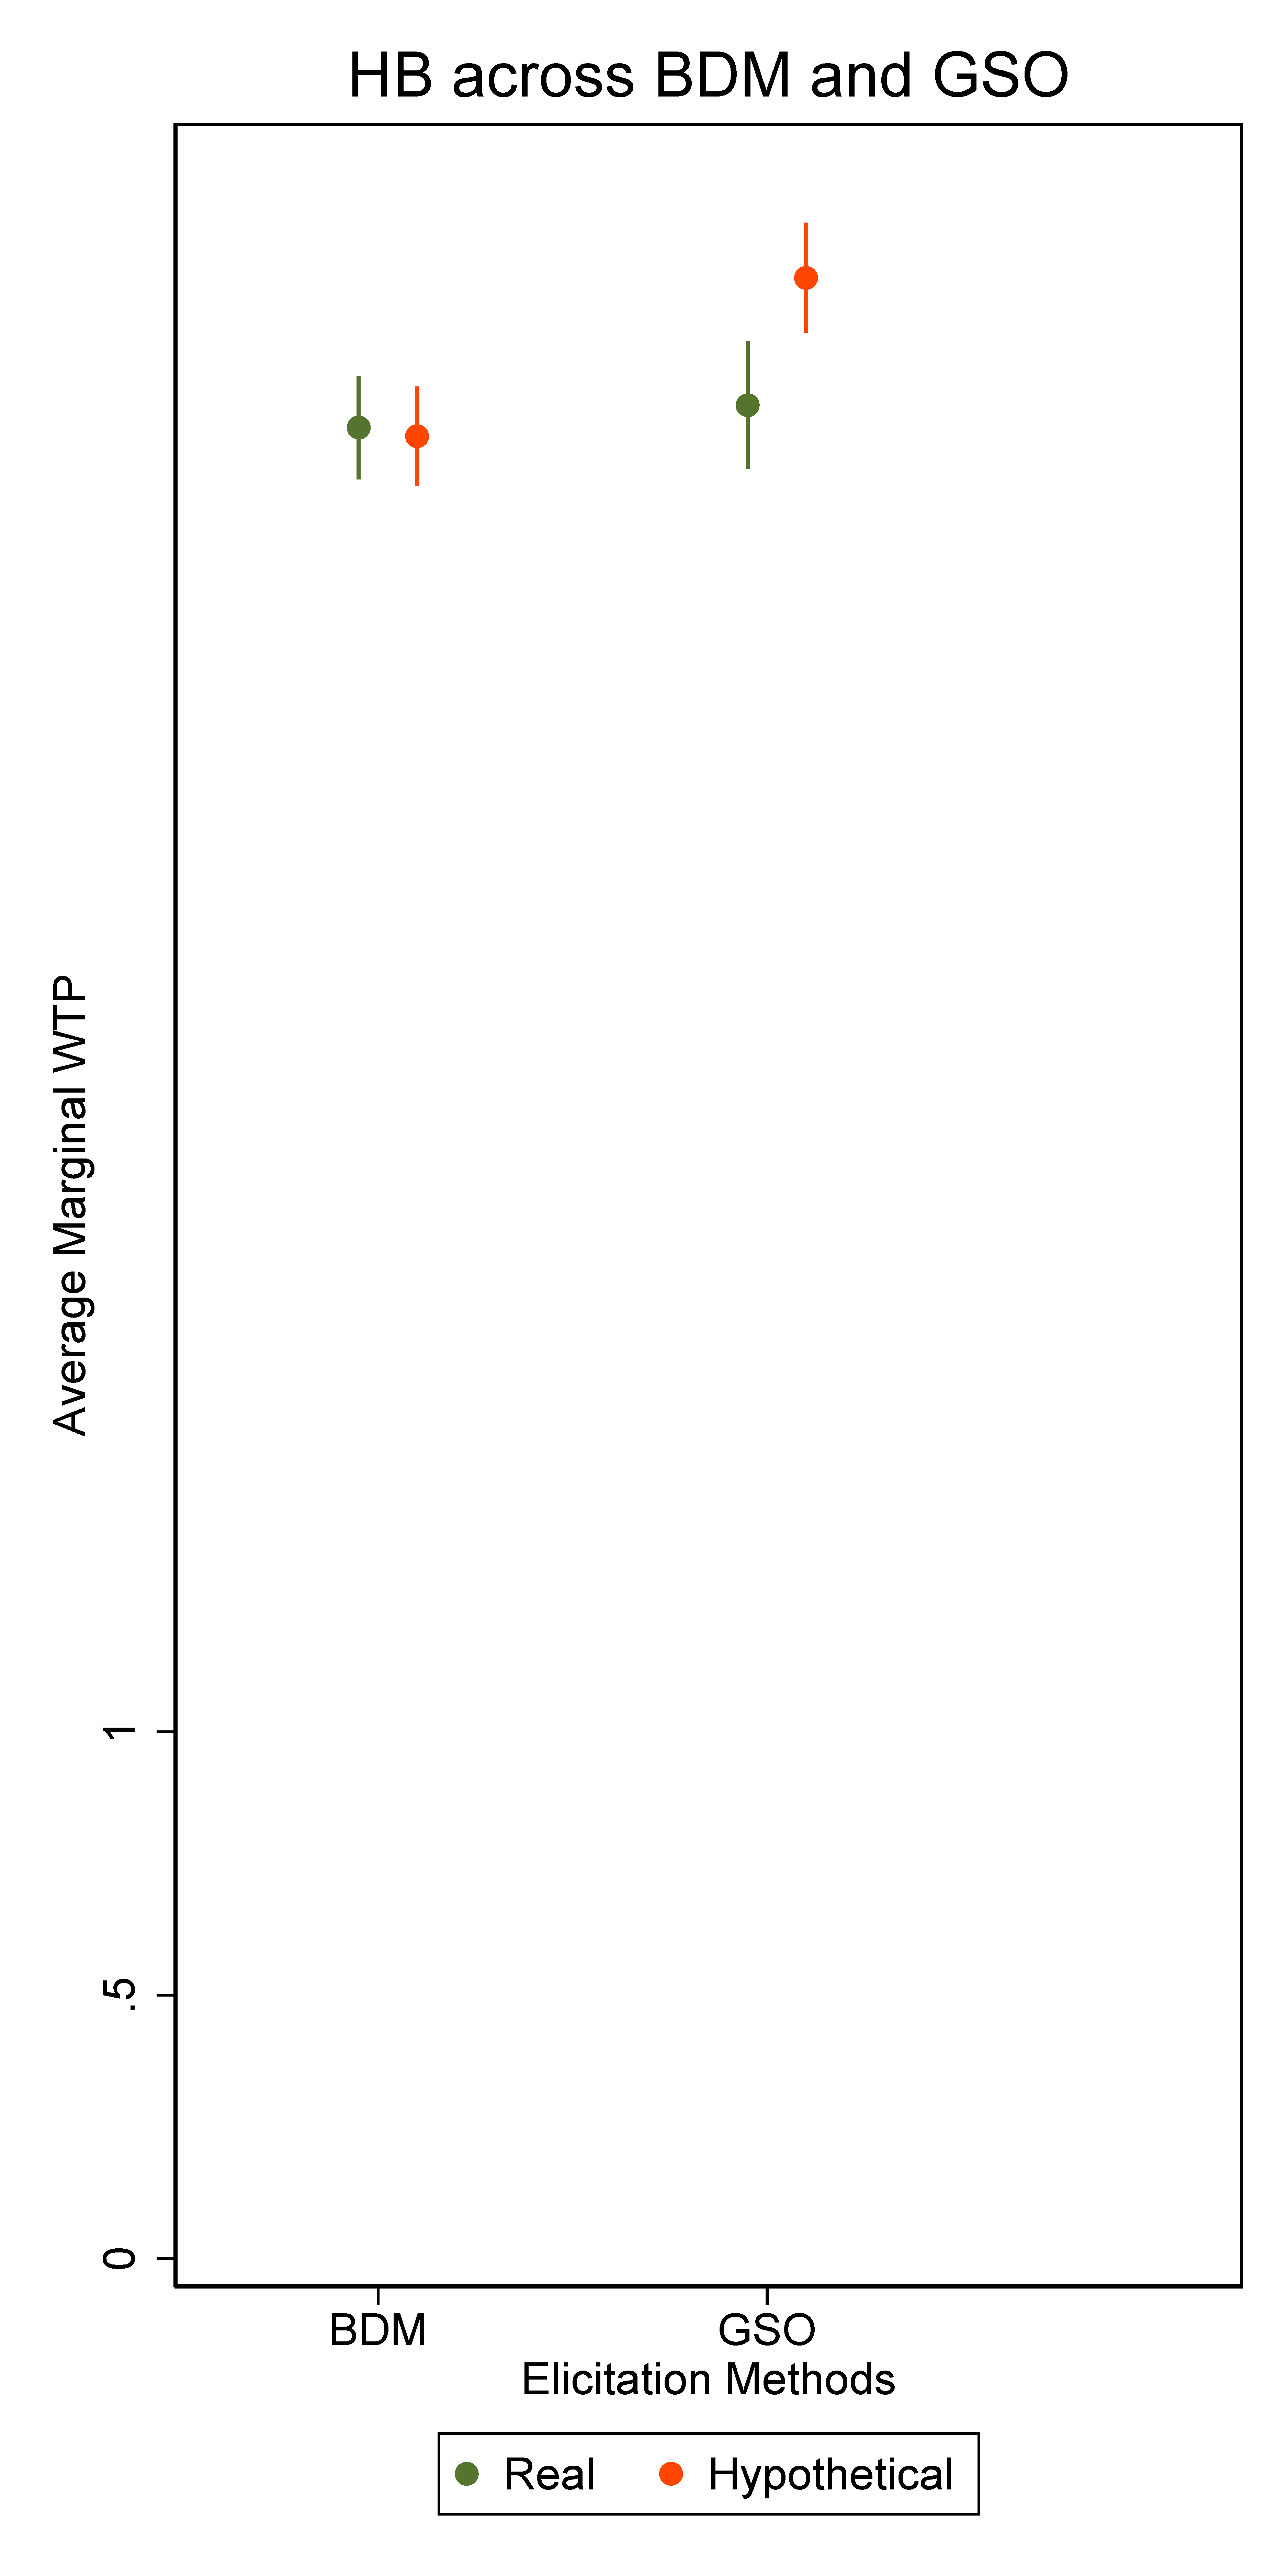
\includegraphics[width=0.7\linewidth]{Model50.pdf}
    \caption{WTP prediction and hypothetical bias}
    \label{fig:margin_hypo}
\end{figure}




\subsection{Summary: Results 1-4}

Given that both elicitation methods perform equivalently under real incentives, and we found that GSO deviates significantly under a hypothetical setting, we can conclude that BDM outperforms GSO in terms of hypothetical bias mitigation. For all preceding results, we also perform parametric and non-parametric tests, such as the multiple comparisons test correcting for Bonferroni, t-test, and the Wilcoxon-Mann-Whitney tests, which all support these results (see Table \ref{tab:mannwhitney} in appendix). We additionally show the distribution of the elicitation methods across the incentives that show thought there may not be significant difference across some comparisons, their distribution may differ.
that show for instance that though the BDM has the same mean value across the treatments, there is a weak evidence that they are not from the same distribution (see Figure \ref{fig:WTP_PDF_CDF_distribution} in appendix).

\hl{I think remove this figure and discussion, it does not add much; we are mostly interested in the marginal effects.}
\begin{figure}[H]
    \centering
    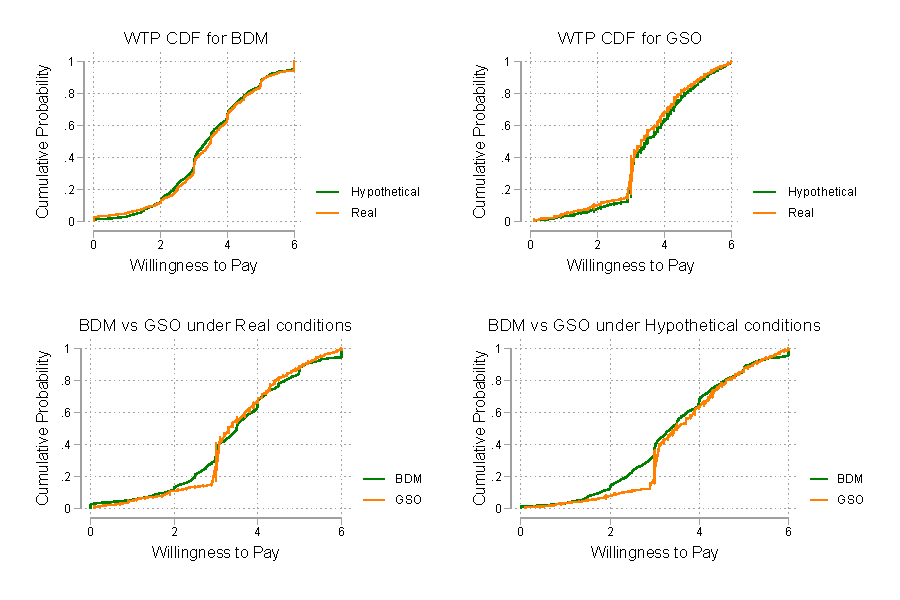
\includegraphics[width=0.8\linewidth]{After_infor_wtp_graph.pdf}
    \caption{Cumulative distribution function (CDF) of WTP across treatments}
    \label{fig:WTP_PDF_CDF_distribution}
\end{figure}



            
\subsection{Mechanism: Sources of hypothetical bias}
\hl{This section is what is going to make the paper interesting. Good job}.

 We first measure whether GSO leads to higher game form recognition as compared to BDM, We conducted a chi-square test to compare proportion of participants who find that the elicitation mechanism is complex in BDM and GSO. The result also confirms that a higher proportion of people in the BDM report high difficulty to understand (see Table \ref{tab:Appendix_proportion_test} in appendix). One might ask why the GSO elicitation method, despite being more game-obvious and perceived as less complex than the BDM method, performs worse in mitigating hypothetical bias. To investigate this puzzle, we examine several contributing factors to the observed difference, including social desirability bias, participants' comprehension of the mechanism, multiple switching behavior, and learning in moderating hypothetical bias over repeated rounds.







\subsubsection{Social desirability}
Social desirability bias is a known contributor to hypothetical bias in stated preference studies \citep{lopez2021social, norwood2011social}, Given the balanced distribution of observable characteristics across treatments, and the absence of hypothetical bias in the BDM condition, we would not expect social desirability to be a major concern in the GSO condition either. However, we examine its potential influence on both mechanisms within our experimental framework. Specifically, we focus on participants who express favorable views toward antibiotic-treated citrus, exhibit hypothetical bias after receiving information on the lethality of the disease and its impact on farmers and citrus orchards. \hl{This is probably endogenous, the comparison may be more fair with one round without information and then adding information that increases the social desirability bias perhaps?} As shown in Table \ref{tab:interval_regression_socialdesirability_BDM} (left-hand side), the results do not indicate that participants with positive attitudes toward genetically modified (GM) products systematically inflate their valuations after receiving that information under neither the GSO (\(\Delta = -0.199\), \(p > 0.10\)) nor the BDM mechanism. This suggests that social desirability does not drive hypothetical bias in the GSO.

\hl{same as before, we only need the marginal effects and coefficients of some key variables like MSB and risk.}
 \begin{table}[H]
        \centering
        \caption{Comparison of Willingness to Pay by Support for Antibiotic Use in Orange Production}
        \label{tab:interval_regression_socialdesirability_BDM}
        \resizebox{0.7\textwidth}{!}{% Scale table to fit the column width
        \begin{tabular}{l*{2}{cc}}
\hline\hline
            &\multicolumn{2}{c}{(1)}           &\multicolumn{2}{c}{(2)}           \\
            &\multicolumn{2}{c}{WTP: GSO (Yes)}    &\multicolumn{2}{c}{WTP: BDM (Yes)}    \\
\hline
Constant    &       3.398\sym{***}&     (0.241)&       3.396\sym{***}&     (0.111)\\
Hypothetical&       0.379\sym{***}&     (0.104)&       0.174\sym{***}&     (0.058)\\
Information&       0.160         &     (0.118)&       0.180\sym{**} &     (0.076)\\
Hypothetical$\times$Information&      -0.199         &     (0.172)&      -0.158         &     (0.110)\\
Risk preferences&      -0.003         &     (0.053)&       0.070\sym{**} &     (0.032)\\
MSB      &       1.135\sym{***}&     (0.161)&                     &            \\
White&      -0.206\sym{*}  &     (0.111)&      -0.235\sym{***}&     (0.057)\\
Middle Income&      -0.425\sym{***}&     (0.108)&       0.155\sym{***}&     (0.059)\\
High Income&       0.175         &     (0.149)&       0.315\sym{***}&     (0.098)\\
Midwest   &      -0.018         &     (0.140)&      -0.149\sym{*}  &     (0.081)\\
South    &       0.186         &     (0.131)&      -0.011         &     (0.075)\\
West    &       0.123         &     (0.155)&      -0.309\sym{***}&     (0.081)\\
Female    &       0.067         &     (0.094)&       0.220\sym{***}&     (0.048)\\
Bachelor&       0.052         &     (0.115)&      -0.051         &     (0.057)\\
No Children  &       0.153         &     (0.101)&       0.156\sym{**} &     (0.067)\\
Maried&       0.012         &     (0.112)&      -0.233\sym{***}&     (0.052)\\
Age         &       0.004         &     (0.003)&       0.007\sym{***}&     (0.002)\\
$\sigma_u$     &       0.931\sym{***}&     (0.049)&       0.998\sym{***}&     (0.023)\\
$\sigma_e$     &       0.865\sym{***}&     (0.053)&       0.830\sym{***}&     (0.025)\\
\hline
\(n\) (observations)       &        1014         &            &        1224         &            \\
\(N\) (subjects)      &        169         &            &        204         &            \\
\hline\hline
\multicolumn{5}{l}{\footnotesize Standard errors in parentheses. * p$<$0.1, ** p$<$0.05 *** p$<$0.01}\\
\end{tabular}
}





\begin{tablenotes}
            \footnotesize
            \item Standard errors in parentheses. * p$<$0.1, ** p$<$0.05, *** p$<$0.01.
            \item \textit{Note:} $\sigma_u$ and $\sigma_e$ denote the standard deviations of the random intercept and residual error, respectively.\\
            $\times$: interaction\\
        \end{tablenotes}
\end{table}



\subsubsection{Participants' understanding of the mechanism and game form recognition}
To examine whether misconceptions contribute to hypothetical bias, we measure whether participants' understanding of the elicitation is a predictor of hypothetical bias. To do so, we use their overall test score in the GSO comprehension assessment task and interact it with hypothetical bias (se table \ref{tab:MSB_interval_regression_Score_overall} in appendix). Our results cannot reject the idea that understanding of the mechanism does not lead to hypothetical bias (\(\Delta = 0.022\), \(p = 0.860\)). In addition, we analyze responses from participants in the top 25\% (highest quartile) and bottom 25\% (lowest quartile) based on their assessment scores (see Table \ref{tab:MSB_interval_regression_Scorehigh_low}). We find that both groups exhibit evidence of hypothetical bias. However, when comparing across conditions, an interesting pattern emerges. In the real setting, participants in the top quartile, those with better comprehension of the BDM mechanism, reported lower valuations, on average about 25 cents less than those in the bottom quartile. This suggests that a better understanding of the mechanism leads to more conservative bidding behavior when decisions carry real consequences. In contrast, in the hypothetical setting, the top-performing group reported valuations approximately \$1 higher than their lower-performing counterparts. As a result, overall hypothetical bias is actually greater among participants with higher comprehension. \hl{This is interesting since it points that better comprehension leads to more hypothetical bias and the GSO is simple so it has better comprehension, so perhaps something to think about and build from}

This pattern suggests that while stronger understanding of the mechanism helps reduce overstatement in real settings, it does not necessarily mitigate and may even exacerbate hypothetical bias when incentives are absent. Although this finding helps illuminate a mechanism behind hypothetical bias, it does not offer a straightforward solution to eliminate the bias.

Finally, as shown in table \ref{tab:Appendix_gameform} in appendix,  we analyze participants perceived complexity of the mechanism, the result suggests that participants in the BDM report a higher level perceived complexity as compared to GSO. Additionally, we measured choice certainty, as how often participants feel like changing their bids. Using this metric, we find GSO leads to a higher choice certainty as compared to BDM. These two results suggests that GSO is more game obvious than BDM as supported by induced value experiment \citep{chakraborty_future_2025,brown_is_2023}.



\subsubsection{Multiple switching behavior}
We first compare participants with and without multiple switching behavior to investigate whether it reflects a preference for randomization (e.g., indecisiveness) or confusion about the mechanism. To explore this, we examine participants' performance and their perceived complexity within the GSO elicitation method, comparing non-multiple switchers to multiple switchers.

A t-test shows no significant differences in test scores between non-switchers and multiple switchers in their assessment test score, suggesting that overall comprehension does not differ meaningfully across these groups. To complement this, we used a chi-square test (see Table \ref{tab:Appendix_proportion_test_groupMSB_vs_Non-MSB}), we find that a significantly higher proportion of MSB participants reported perceiving the mechanism as highly complex compared to non-MSB participants (\(\Delta = 14\%\), \(p < 0.001\)). This suggests that multiple switching may be more a result of confusion rather than of a deliberate preference for randomization.


Finally, we assess whether multiple switching contributes to hypothetical bias, we create a dummy variable indicating MSB  and interact it with the incentive condition. The results (Table \ref{tab:MSB_interval_regression_MSB}, Appendix) indicate that MSB does not significantly influence hypothetical bias (\(\Delta = 0.14\), \(p > 0.10\)). We further validate this finding using three model specifications: (1) including all participants, (2) excluding multiple switchers, and (3) analyzing only multiple switchers (see Table \ref{tab:MSB_interval_regression_multiple_comaparisons} in the Appendix). While results indicate valuation inflation among multiple switchers under both real and hypothetical scenarios, we find no statistical evidence that multiple-switching behavior drives the hypothetical bias observed in the GSO mechanism. Therefore, multiple switching can be ruled out as the primary source of hypothetical bias in this study.

In summary, multiple switching does not appear to reflect a fundamental misunderstanding of the mechanism, nor does it exacerbate hypothetical bias. Rather, it may be associated with valuation inflation, possibly indicating lower-quality responses among those participants.




\subsubsection{Attention in the tasks}

Following \citet{chabris2008measuring}, we measure response deliberation time in elicitation tasks to assess whether this hypothetical bias in the GSO is driven by that. Specifically, we use the time per increment that we obtain by standardizing the number of decisions faced by each participant, we divide the final price at which the game ends by 0.2. This gives a consistent measure of the number of increments each participant encountered, since each increment corresponds to an increase of \$0.20 increase. In other words, when the random price is \$X, the participant faced 5X increments decisions. Given that participants are not paid in the hypothetical treatments, if this was the driver of hypothetical bias, if lack of attention was a driver of hypothetical bias, we would expect them to spend significantly less time in the hypothetical treatment. Doing a t-test we found the opposite in the GSO, participants in the hypothetical treatment group spend on average 10\% more time than in real one (see table \ref{tab:my_label} in the appendix).  However, in the BDM, we found no statistical different between real and hypothetical treatments. Hence, we can omit selective attention as driver of hypothetical bias found in the GSO.










\subsubsection{Learning in GSO decreases hypothetical bias}
As shown, in Table \ref{tab:interval_regression_RounbyRound} and Figure \ref{fig:HB Round by Round}, We analyze hypothetical bias round by round to see whether learning can contribute to mitigating hypothetical bias gap. For BDM, there is no evidence of learning leading to changes of bidding behavior, the bids are relatively stable across the rounds.
For GSO, focusing on Round 1, we observe that the hypothetical bias is the highest (\(\Delta = 0.326\), \(p < 0.01\)). In Round 2, there is evidence of learning, as the hypothetical bias decreases by 37\% (\(\Delta = 0.238\), \(p = 0.001\)). In Round 3, there is no evidence of hypothetical bias in GSO (\(\Delta = 0.21\), \(p = 0.007\)). consistent with \citet{brown_is_2023}. Using the predicted value showing in the figure, it suggests no difference at 5\%. Overall, we find that that participants learn to play their weakly dominant strategy over the rounds. \footnote{Comparing GSO and BDM across incentive settings, we find that under the non-hypothetical setting, BDM and GSO are not systematically different across rounds. However, under the hypothetical setting, GSO and BDM remain systematically different, although the gap decreases over the rounds—from \$0.47 to \$0.23. (see Table \ref{tab:MSB_interval_regression_multiple_comaparisons} in appendix).}







\hl{same comment as before about the x-axis and y-axis. What does this figure show? Predicted wtps? Are the bars CIs? I think we should show marginal effects. The discussion in the text is not connected to the figure so what is the usefulness of the figure?}
\begin{figure}[H]
    \centering
    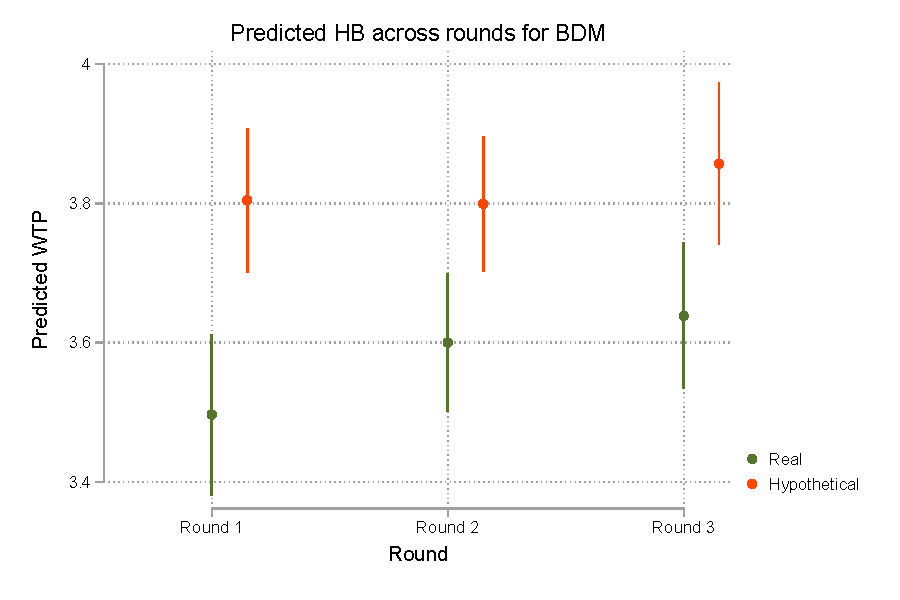
\includegraphics[width=0.7\linewidth]{Model110.pdf}
    \caption{Hypothetical bias (HB) across rounds}
    \label{fig:HB Round by Round}
\end{figure}










\subsubsection{Discussion}

Other factors driving hypothetical bias according to the literature are strategic misrepresentation \citep{meginnis2021strategic}, social desirability \citep{lopez2021social, norwood2011social} and consumer and product characteristics \citep{hofstetter2013consumer}. We can omit this mechanism since all of these are the same within both BDM and GSO and given that our data is well balanced. \hl{Another approach is to test them all... we do have social desirability and product characteristics... see my comment about social desirability.. and the products} Another possibility is lack of clarity, we measured participants score following the instructions. We found that it does not help to address hypothetical bias gap noticed in the GSO, neither does it differ among multiple switchers and non-switchers supporting \citet{yu2021multiple} who found that cognitive ability is not predictive of MSB. However, we found suggestive evidence that selective attention is the major predictor of hypothetical bias in the GSO, aligning with \citet{yu2021multiple}. Notably, our results also show that learning significantly improves decision quality in the GSO, whereas we find no such evidence of learning effects in the BDM.


\hl{I stopped here as I feel we are trying to do two papers and fit them into one, and perhaps we are better off doing two separate papers.}


\section{Robustness analysis}

As a robustness check, we run similar analysis as the previous one in the result section by excluding multiple switchers. The results are robust to the exclusion of multiple switchers. (see Table \ref{tab:MSB_interval_regression_multiple_comaparisons} in appendix). 
 




\section{Conclusion}

In this study we address the fundamental question of how GSO, an elicitation known to be game obvious, performs as compared to BDM (a largely used preference elicitation method) in real consumer valuation contexts in hypothetical bias mitigation. The experiment involved a randomized online survey, participants were assigned to one of four treatment groups: GSO with real incentives, GSO hypothetical, BDM with real incentives, and BDM hypothetical. Our results show that, as predicted by theory, GSO is more game-obvious than BDM—that is, participants more easily understood the incentives involved. However, BDM outperformed GSO in mitigating hypothetical bias. Interestingly, the two mechanisms perform equivalently when real incentives were provided. Moreover, we find that participants in GSO learn to bid valuation over rounds that help bridging hypothetical bias gap, while for BDM, participants' bids remain stable over the rounds. This indicates that GSO's transparent structure facilitates strategy discovery, allowing participants to converge toward truthful revelation through experience—a valuable property for multi-round experimental protocols.  While BDM may be a more effective mechanism when participants have higher levels of formal education, this advantage may not hold in contexts where individuals often lack such education or familiarity with economic mechanisms like randomization procedures, such as in many developing countries\citep{burchardi2021testing, akbarpour2020credible}. In these settings, GSO may be more appropriate, as it perceived to be less complex and facilitates learning over time, as demonstrated in this study.


Our findings have important methodological implications for mechanism design and experimental economics. First, the relationship between a mechanism’s obviousness and its ability to elicit truthful valuations is non-monotonic. While simplification can enhance comprehension such as in the case of GSO, excessive simplicity, particularly in the absence of real incentives may trigger heuristic decision-making, leading to noise rather than accuracy. This highlights the need for careful design calibration, balancing clarity with enough structural complexity to maintain participant engagement and reflective responses. Second, the GSO mechanism may be particularly well-suited to experimental contexts that involve multi-stage bidding. Its intuitive structure appears to support learning, allowing participants to gradually identify their best responses over successive rounds. In such settings, GSO offers a promising approach for promoting strategy-proof behavior, especially when participants are unfamiliar with more abstract elicitation formats like BDM. Overall under hypothetical scenario, our result suggests BDM is more reliable. However under real setting, especially when there is an opportunity to learn the mechanism more through repeated rounds, the GSO would be recommended more than the BDM. 

One limitation of the study that merits consideration is that it is unclear whether GSO's learning advantages compound over many rounds or plateau after initial strategy discovery. In our case, since information was introduced before the third round, it may interact with learning.
Two promising avenues emerge from this work. Examining these mechanisms' performance across different contexts (e.g., different product categories, different stakes, environments) would test the robustness of our findings. 


\bibliography{Refer_Antibiotics}


\newpage
	\singlespacing
	\appendix
	\setcounter{table}{0}
	\setcounter{figure}{0}
	\renewcommand{\thetable}{A\arabic{table}}
	\renewcommand{\thefigure}{A\arabic{figure}}
	\setcounter{page}{1}
	\renewcommand{\thesubsection}{\Alph{subsection}}

	\section*{\centering{Electronic Supplementary Material of}}
	{\centering \LARGE Game structure obviousness in homegrown preference elicitation
		
		\vspace{0.5cm}
		\renewcommand*{\thefootnote}{\fnsymbol{footnote}}
		\setcounter{footnote}{0}
		
		\large
        
\section{Research protocol}

Welcome to a study of how people make economic decisions!Please read the instructions carefully and click the continue button if you agree with the Informed Consent below.

\textbf{Title of Research Study}: Consumer economic decision-making

\textbf{Investigator}: Dr. Samuel Zapata\par

\textbf{Why am I being asked to take part in this research study?}\par

You are invited to participate in this study because we are trying to learn more about consumers' preferences for beef. You were selected as a possible participant in this study because you are a U.S. consumer. You must be 18 years of age or older to participate. \par
\textbf{Why is this research being done?} \par

The survey is designed to understand consumer economic decision making. \par

\textbf{How long will the research last?} \par
It will take about 15 minutes. \par
\textbf{What happens if I say "Yes, I want to be in this research"?} \par
If you decide to participate, you will be asked to provide your valuations for several products and answer a survey. \par


\textbf{
What happens if I do not want to be in this research?} \par
Your participation in this study is voluntary. You can decide not to participate in this research and it will not be held against you. You can leave the study at any time. \par

\textbf{Is there any way being in this study could harm me?}
There are no sensitive questions in this survey that should cause discomfort. \par

\textbf{What happens to the information collected for the research?} \par
You may view the survey host’s confidentiality policy at: \href{https://www.beforthright.com/privacy}{Forthright Privacy Policy}. Your email address or other contact information will be stored separately from your survey data, and is only being collected for those who purchase products so we can mail them their products to their designated mailing address. All identifiable information will be kept on a password protected computer and is only accessible by the research team. Compliance offices at Texas A\&M may be given access to the studies files upon request. Your information will be kept confidential and allowed by law. The results of the research study may be published but your identity will remain confidential. \par

\textbf{Will my information be used for other research?} \par
Information collected as part of the research will NOT be used for other studies or given to other researchers for future studies. \par

\textbf{What else do I need to know?} \par

If you agree to take part in this research study, we will provide you with  \$3 compensation and may earn additional compensation in cash or a food product that, if eligible, will be mailed to you at the mailing address you designated within a week after completing the study. This is optional if you do not want to provide your email address or a mailing address. \par

\textbf{Who can I talk to?} \par

Please feel free to ask questions regarding this study. You may contact me later if you have additional questions or concerns at 1-979-845-5284 and mapalma@tamu.edu, Dr. Marco Palma. You may also contact the Human Research Protection Program at Texas A\&M University (which is a group of people who review the research to protect your rights) by phone at 1-979-458-4067, toll-free at 1-855-795-8636, or by email at irb@tamu.edu for:\par

\begin{itemize}
    \item Additional help with any questions about the research.
    \item Voicing concerns or complaints about the research.
    \item Obtaining answers to questions about your rights as a research participant.
    \item Concerns in the event the research staff could not be reached.
    \item The desire to talk to someone other than the research staff.
\end{itemize} \par



If you want a copy of this consent for your records, you can print it from the screen. \par

I freely agree to participate in this study \par
[Dropdown menu options:] \par
Yes, I agree \par

No, I don't agree and want to terminate the study

\section{Online experiment}

 Please indicate how often you consume oranges and similar fruits like tangerines, grapefruits, and mandarins (Screen out if last two categories).  

\begin{itemize}
    \item Daily
    \item 3-4 times a week
    \item Once a week
    \item 2-3 times a month
    \item Once a month
    \item Rarely or Never
\end{itemize}

\vspace{1cm} % Adds spacing before the warning

\textbf{Warning:} This study contains quality checks. You might be excluded at any point of the study if you do not pass quality checks or if you are not paying attention.


\clearpage


\subsection{BDM Hypothetical}

\subsubsection*{Instructions }


For this study, we will explore your preferences for oranges. \textbf{You will only receive a participation fee of \$2.00}. \par

 In the next screen you will be presented with a hypothetical scenario. Note that the scenario is hypothetical, but we ask you to make your decisions as if you were in a real market using real money. \par

Although we will describe the rules of the procedure shortly as if it actually involves money, you will not actually have to pay anything, and we will not ship any products to you. \par

However,\textbf{ we do want you to treat it as if it was real}. That is, although you will not receive a bag of oranges and you will not actually have to pay anything, we still want you to formulate your bid thinking what you would do if you had to do it for real. \par

You will receive more details about this procedure below.

\clearpage



\subsubsection*{Instructions (continued)}

In this study, you will complete 3 Tasks and a survey.

For each task, you will be endowed with a card with a value of \$6.00. You can use the funds in the card to purchase a bag of oranges (3.2 lbs – approximately 6-8 oranges) in two distinct markets. Any remaining funds in the card that you don’t spend on the oranges will be added to your earnings on top of your \$2.00 participation fee if you are selected for payment.



In one market, the oranges are from trees treated with antibiotics by injection to the *tree’s trunks* (not directly in the orange fruits) to prevent yield and fruit quality losses caused by a disease called citrus greening. The other market is conventional oranges, not from trees treated with antibiotics, but using a combination of pesticides and cultural practices.

You can use the funds in your card to bid on one of the markets or both. Your bid will be compared to an unrelated fixed price that is equally likely to be a number between $0.00 and $6.00. If your bid is higher than the fixed price, you will purchase the item. But here is the interesting part, in this case, you do not pay the price you offer, instead you pay the fixed offer. If your bid is lower than the fixed price, you do not buy the orange and you do not pay anything. 

\vspace{0.5cm}

\textbf{\underline{Please remember this decision is hypothetical and you will not earn money or a bag of oranges.}} 

In each market (see below), you can choose the maximum amount you are willing to pay for a bag of oranges.
\clearpage

\subsubsection{\textbf{Instructions (continued)}}
 Here is a practice screen to familiarize yourself with the slider. Your responses here will not count toward the main study.

\begin{figure}[H]
    \centering
    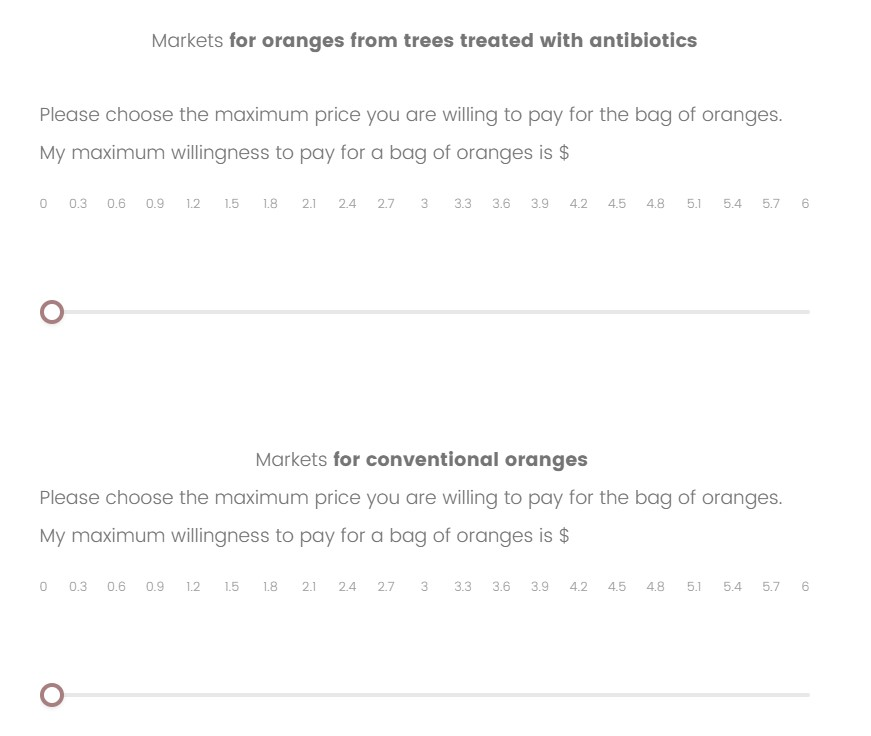
\includegraphics[width=0.8\linewidth]{BDM_market.jpg}

\end{figure}

\clearpage

\definecolor{navyblue}{RGB}{0, 0, 128}

\subsubsection*{Instructions (continued)}
Let me give you an example: Assume that you bid \textbf{\$3.00}, and the fixed price is \textcolor{cyan}{\$2.80}, then you win the orange and only pay \textcolor{cyan}{\$2.80}. If, however, your price was lower than the fixed price, then you do not buy the orange.  

You should offer the maximum price you are willing to pay for the orange; there are no advantages to strategic behavior in this task. Your best strategy is to determine your personal value for the orange and offer that price.  

\vspace{0.3cm}

\textbf{Why is it my best strategy to bid the maximum price I’d be willing to pay?}  

If I truly value the orange at \textbf{\$3.00}, however instead of bidding \textcolor{orange}{\$3.00}, I bid \textcolor{orange}{\$2.60}, and the fixed price is \textcolor{cyan}{\$2.80}, then I lose the opportunity to purchase the oranges. However, had I bid my true valuation I would have won and paid only \textcolor{cyan}{\$2.80} for an orange I think is worth \textbf{\$3.00}.  

Now what if I offer more? Let’s say that I truly valued the orange at \textbf{\$3.00} and I bid \textcolor{orange}{\$5.00}, and the fixed price ended up being \textcolor{orange}{\$4.40}. Then I win, I will have to pay \textcolor{cyan}{\$4.40} for an item I value at \textbf{\$3.00}.  

\vspace{0.5cm} 

When you have understood the instructions, please proceed to the next page.  


\clearpage


\subsubsection*{Instructions continued}


\textbf{Example 1}: If the card you own can be redeemed for a bonus of \$6.00, you bid \$3.00 and the fixed price is \$2.40, you have a higher bid than the fixed price. You buy the item, and you pay the fixed price (\$2.40), plus your balance is (\$6.00 - \$2.40 = \$3.60) and you get the product which will be shipped to your specified mailing address using priority shipping.
\vspace{0.5cm}


\textbf{Example 2}: If the card you own can be redeemed for a bonus of \$6.00, your bid is \$3.00 and the fixed price is \$4.00, you have a bid lower than the fixed price. You do not buy the item, and you receive your bonus of \$6.00.

\vspace{0.5cm}

When you have understood the instructions, please proceed to the next page.
\clearpage


\subsubsection*{Comprehension test}
Note: All following questions will provide simple explanations if the subject indicates or types the wrong answer(correct answer is in bold).

\vspace{0.5cm}

True or False? The fixed price will be a known number to me before I make a decision.  

• True  \par
\textbf{• False}\par  

\vspace{0.5cm}


\vspace{0.5cm}



True or False? My best strategy is to bid the maximum I'd be willing to pay.  

\textbf{• True}  \par
• False 

\vspace{0.5cm}

If I value both oranges at \$5.00:

\textbf{a) Although the value of my card is less than \$10.00, I can bid \$5.00 in each market. However, only one of these bids will be binding.}  

b) I can only bid in one market since the value of my card is less than \$10.00.  

\vspace{0.5cm}

If the card you own could be redeemed for a bonus of \$6.00, your bid was \$4.00 and the fixed price was \$2.4, what would have been your final outcome?  

\textbf{a) I pay \$2.40 for the orange, so my balance is \$6 - \$2.40 = \$3.60 } 

b) The value of my card is \$6.00, since I cannot buy the orange  

c) I pay \$4.00 for the orange, so my balance is \$6.00 - \$4.00 = \$2.00  

\vspace{0.5cm}

If the card you own could be redeemed for a bonus of \$6.00, your bid is \$3.40 and the fixed price is \$4.00, what would be your final outcome?  

d) I pay \$4.00 for the orange, so my balance is \$6.00 - \$4.00 = \$2.00  

\textbf{e) The value of my card is \$6.00, since I cannot buy the orange } 

f) I pay \$3.4 for the orange, so my balance is \$6.00 - \$3.40 = \$2.60  

\vspace{0.5cm}

\subsubsection*{\textbf{Instructions (continued)}}

You have successfully completed the comprehension test, and you will now begin Task 1.\par

\vspace{0.5cm}
 Please click next when you are ready to proceed.

Now, we will go to the main tasks. \par
\textbf{\underline{Please remember this decision is hypothetical and you will not earn money or a bag of oranges.}}

\clearpage

\subsubsection*{\centering \textbf{Round 1 \& 2}}

\begin{figure}[H]
    \centering
    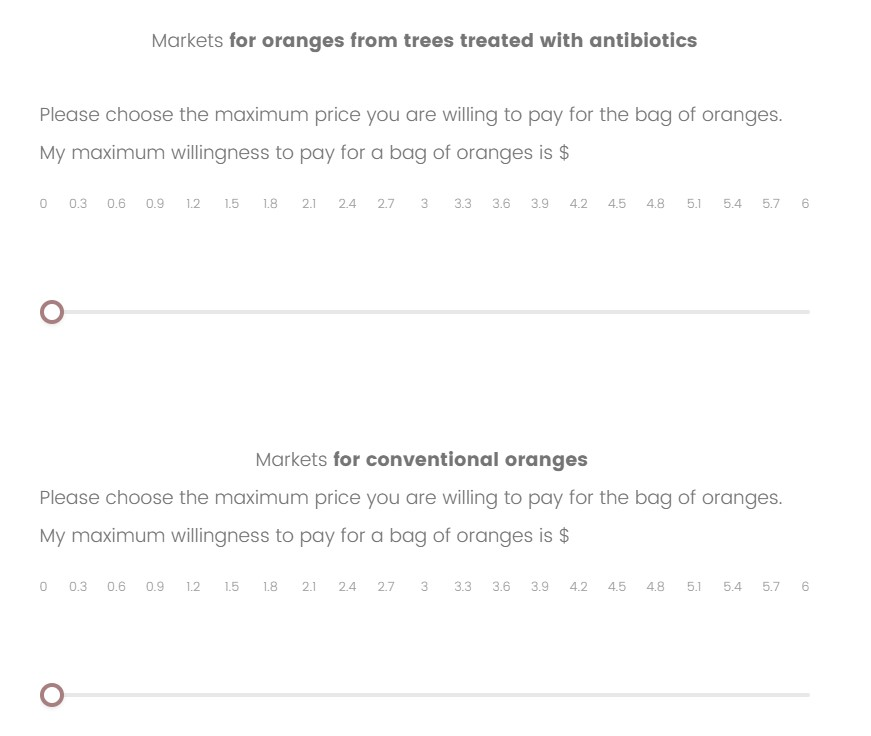
\includegraphics[width=0.8\linewidth]{BDM_market.jpg}
    \caption{dd}
    \label{fig:BDM_market}
\end{figure}

\clearpage

\subsubsection*{\textbf{Instructions (continued)}}
On the next page, you will see a video. \textbf{Please ensure your speakers or headphones are connected and the volume is set properly.} Next you will see a video that provides information about a disease Watch the video carefully in a quiet, distraction-free environment, as it is essential for the study.
\vspace{0.5cm}
Click on the video to watch it.

\href{https://www.youtube.com/watch?v=_AqMBjB0ChM}{video}
\clearpage


 \subsubsection*{\centering Round 3}


\begin{figure}[H]
    \centering
    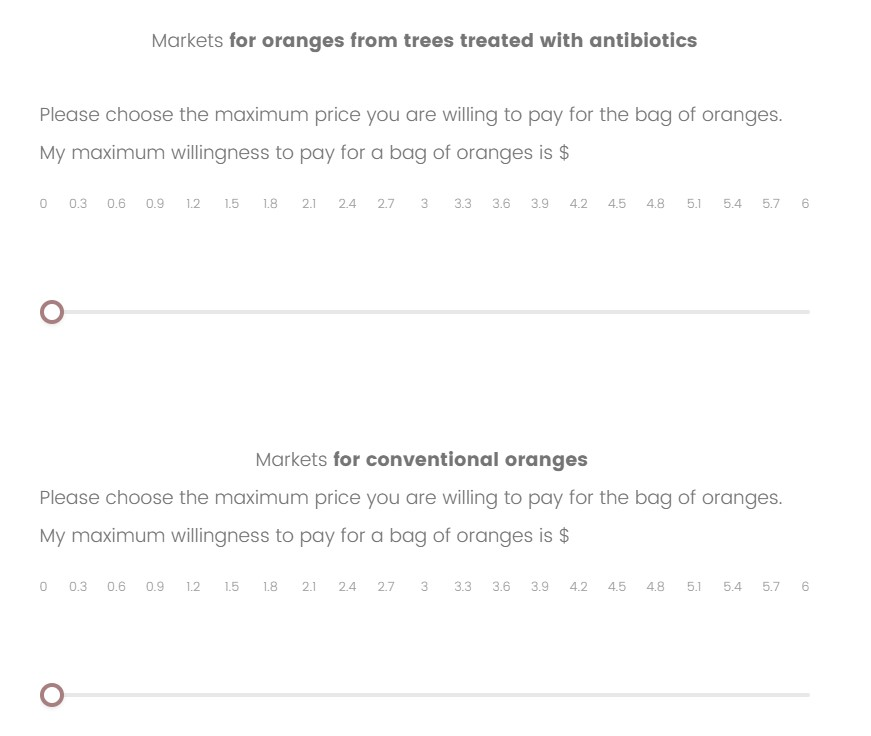
\includegraphics[width=\linewidth]{BDM_market.jpg}
    \caption{}
    \label{fig:BDM_market}
\end{figure}

\clearpage



\subsection{BDM Real}


\subsubsection*{\textbf{Instructions (continued)}}


For this study you will receive a fixed fee of \$2 and you can earn additional compensation in cash and/or citrus products based on your decisions and chance, so please pay attention to the instructions.
 
You will complete 3 Tasks that involve real money, so please pay attention to the instructions. There is a 10\% chance that your decisions will be selected for payment. After completing the 3 tasks, the computer will draw a random number between 1 and 10. If the random number is equal to 1, you will receive the payoff as described below. However, if the random number is between 2 and 10, your decision will not yield additional earnings, and you will receive just the \$2. If you are selected for payment, one of the three tasks will be randomly selected to be added to your compensation.

 Since there is a chance that your decision will end up affecting your earnings, it is in your best interest to respond carefully to each task. If your compensation includes a food product (oranges), the product will be shipped to your specified address *free of charge* via priority mail as long as you provide us with a valid mailing address. You will receive more details about this procedure below.

\clearpage

\subsubsection*{\textbf{Instructions (continued)}}

In this study, you will complete 3 Tasks and a survey.
For each task, you will be endowed with a card with a value of \$6.00. You can use the funds in the card to purchase a bag of oranges (3.2 lbs – approximately 6-8 oranges) in two distinct markets. Any remaining funds in the card that you don’t spend on the oranges will be added to your earnings on top of your \$2.00 participation fee if you are selected for payment.



In one market, the oranges are from trees treated with antibiotics by injection to the *tree’s trunks* (not directly in the orange fruits) to prevent yield and fruit quality losses caused by a disease called citrus greening. The other market is conventional oranges, not from trees treated with antibiotics, but using a combination of pesticides and cultural practices.


You can use the funds in your card to bid on one of the markets or both. Your bid will be compared to an unrelated fixed price that is equally likely to be a number between $0.00 and $6.00. If your bid is higher than the fixed price, you will purchase the item. But here is the interesting part, in this case, you do not pay the price you offer, instead you pay the fixed offer. If your bid is lower than the fixed price, you do not buy the orange and you do not pay anything. 

 

\textbf{ \underline{Please remember this decision is real and you may earn money or any bag of oranges.}}

 

 \clearpage

\subsubsection*{\textbf{Instructions (continued)}}

From that point, the instructions are the same as hypothetical, with a different reminder as shown below;

 Now, we will go to the main tasks.


\textbf{ \underline{Please remember this decision is real and you may earn money or any bag of oranges.}}

 \clearpage

 \subsection{GSO Hypothetical}
 \subsubsection*{\textbf{Instructions (continued)}}

For this study, we will explore your preferences for oranges. You will only receive a participation fee of \$2.00. In the next screen you will be presented with a hypothetical scenario. Note that the scenario is hypothetical, but we ask you to make your decisions as if you were in a real market using real money. Although we will describe the rules of the procedure shortly as if it actually involves money, you will not actually have to pay anything, and we will not ship any products to you. However, we do want you to treat it as if it was real. That is, although you will not receive a bag of oranges and you will not actually have to pay anything, we still want you to formulate your bid thinking what you would do if you had to do it for real. You will receive more details about this procedure below.


\clearpage

\subsubsection*{\textbf{Instructions (continued)}}

In this study, you will complete 3 Tasks and a survey.

For each task, you will be endowed with a card with a value of \$6.00. You can use the funds in the card to purchase a bag of oranges (3.2 lbs – approximately 6-8 oranges) in two distinct markets. Any remaining funds in the card that you don’t spend on the oranges will be added to your earnings on top of your \$2.00 participation fee if you are selected for payment.

In one market, the oranges are treated with antibiotics by injection to the *tree’s trunks* (not directly in the orange fruits) to prevent yield and fruit quality losses caused by a disease called citrus greening. The other market is conventional oranges, not treated with antibiotics, but using a combination of pesticides and cultural practices.

You can use the funds in your card to purchase from one of the markets or both.

 
\textbf{\underline{Please remember this decision is hypothetical and you will not earn money or any bag of oranges.}}

\clearpage

\subsubsection*{\textbf{Instructions (continued)}}

 In each market, offer prices will be displayed on the screen, and you will make choices over several periods. For every period, you can click “Try to Buy” if you are willing to buy the bag of oranges at the corresponding offer price or click “Not Buy” if you are not willing to buy at that offer price.
The computer has already randomly chosen the \textbf{market price} at which it will accept to sell the bag of oranges to you. That price is drawn between \$0.00 and \$6.00 and is equally likely.

In the first period, the offer price starts at \textcolor{orange}{\$0.00 }and will increase by \$0.20 after every period. The task ends when the price on the screen increases to the \textbf{market price} that the computer chose to sell the bag of oranges.
At every other price, whether you choose “Try to Buy” or “Not Buy”, you will go to the next period and again choose between “Try to Buy” or “Not Buy”.
The task will continue until the offer price reaches the market price the computer chose to try to sell the bag of oranges to you. At that price:

\begin{enumerate}
    \item If you choose “Try to Buy”, you receive the market price, and task ends.
    \item If you choose “Not Buy” you will not be able to buy the bag of oranges and task ends.
\end{enumerate}


For example, let’s say you are in Period 1, when the offer price is \$0.00. If the computer tries to sell you the bag of oranges at that price, and you click “Try to Buy”, you will get the bag of oranges at the current price \$0.00. If instead you clicked “Not Buy”, you will not be able to buy the bag of oranges. However, if the computer does not try to sell you the bag of oranges at that price, you will go to the next period.

\clearpage



\subsubsection*{\textbf{Instructions (continued)}}


Here is a practice screen to familiarize yourself with the buttons or with the way you choose to buy or not buy. Your responses here will not count toward the main study.
Please keep making choices until the buttons turn red, that is when then the market is over.

\begin{figure}[H]
    \centering
    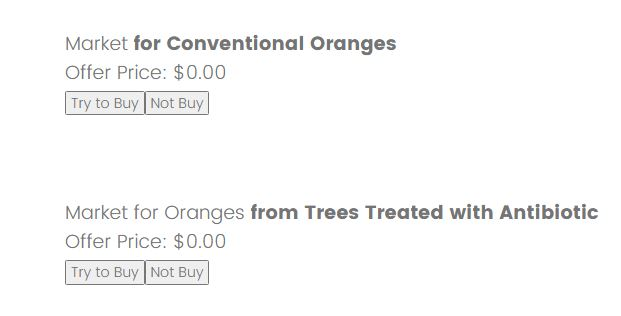
\includegraphics[width=0.8\linewidth]{GSO.JPG}
    
    \label{fig:GSO}
\end{figure}

\clearpage


\subsubsection*{\textbf{Instructions (continued)}}

\textbf{Example 1}

Suppose the maximum amount \textbf{Person X} is willing to pay for the bag of oranges is \textbf{\$3.00}. The first offer price starts at \textcolor{orange}{\$0.00}. Since Person X is willing to purchase the bag of oranges for \textcolor{orange}{\$0.00} (because Person X is willing to pay up to \$3.00), then He/ She would click “Try to Buy” at that offer price.

Suppose the randomly drawn \textbf{market price} from \$0.00 to \$6 is \$2.00 (you will not be able to see it), since the offer price is lower than the market price, Person X would not be able to buy the bag of oranges when selecting “Try to Buy”. He/ She will proceed to the next period where offer price will be \textcolor{orange}{\$0.20}.
Since Person X is willing to purchase the bag of oranges at \$0.20, He/ She would select “Try to Buy”. Once again, the offer price will be compared to the market price. Since the randomly drawn market price in our example was \$2.00, Person X would not buy the bag oranges and He/ She will proceed to the next offer price of \textcolor{orange}{\$0.40}.


This process will continue until the offer price is \textcolor{orange}{\$2.00}. When the offer price is \textcolor{orange}{\$2.00}, Person X chooses “try to buy” and since the market price is \textcolor{cyan}{\$2.00} a transaction will occur at that time. Note that Person X maximum willingness to pay for the bag of oranges was \textbf{\$3.00}, but the market price randomly generated by the computer was \textcolor{cyan}{\$2.00}. So, if selected for payment, Person X would purchase the bag of oranges and receive them via priority shipping to their designated mailing address and the remaining \$4.00 on their card will be added to their compensation.



Please proceed to the next page for another example.
\clearpage

\subsubsection*{\textbf{Instructions (continued)}}

Example 2

Suppose the maximum amount \textbf{Person X} is willing to pay for the bag of oranges is \textbf{\$3.00}. The first offer price starts at \textcolor{orange}{\$0.00}. Since Person X is willing to purchase the bag of oranges for \textcolor{orange}{\$0.00} (because Person X is willing to pay up to \$3.00), then He/ She would click “Try to Buy” at that offer price.

Suppose the randomly drawn market price from \$0.00 to \$6.00 is \textcolor{cyan}{\$4.00} (you will not be able to see it), since the offer price is lower than the market price, Person X would not be able to buy the bag of oranges when selecting “Try to Buy”. He/ She will proceed to the next period where offer price will be \textcolor{orange}{\$0.20}.

Since Person X is willing to purchase the bag of oranges at \textcolor{orange}{\$0.20}, He/ She would select “Try to Buy”. Once again, the offer price will be compared to the market price. Since the randomly drawn market price in our example was \textcolor{cyan}{\$4.00}, Person X would not buy the bag oranges, and He/ She will proceed to the next offer price of \textcolor{orange}{\$0.40}.


This process will continue until the offer price is \textcolor{orange}{\$3.00}.  However, in the next round, the offer price will be \textcolor{orange}{\$3.20}. When the offer price is \textcolor{orange}{\$3.20}, Person X would click “Not buy”. When clicking “Not buy”, she will go to the next round and will continue to click “Not Buy” until task ends and will not be able to buy the bag of oranges. In this example, task ends when the offer price reaches \textcolor{cyan}{\$4.00}. Person X will click “Not Buy” at this price and will not be able to buy the bag of oranges.
\vspace{0.5cm}

When you have understood the instructions, please proceed to the next page.
\clearpage

\subsubsection*{Comprehension test}

Select which statement below is the most correct

\begin{itemize}
    \item The price increases by \$0.20 in each subsequent period 
    \item The value of your card does not change
    \item \textbf{Both answers are true}
\end{itemize}

\vspace{0.5cm}

What will happen to your reward if you try to buy when the fixed price is \$4.40, and the computer accepts your price?

\begin{itemize}
    \item I will get \$6, which is the value of my card
    \item \textbf{I will pay the oranges at \$4.40, plus get my balance of \$6.00-4.40=\$1.60}
    \item It is random
\end{itemize}

\vspace{0.5cm}


If the price of oranges in both markets is \$5.00 at a given period, can I try to buy both oranges in both markets?

\begin{itemize}
    \item No, you can’t because your card is worth \$6, it exceeds your endowment.
    \item \textbf{Yes, you can, however if the computer accepts both prices, only one decision will be randomly binding for realization.}
\end{itemize}

\vspace{0.5cm}

If Person' X maximum willingness to pay for the orange is \$3.00, S/He would switch from "Try to Buy" to "Not Buy" at \$3.20.

\begin{itemize}
    \item \textbf{Then Person X will continue to click "Not Buy" until the market ends}
    
    \item Person X should try to switch back and forth to "Try to Buy" and "Not Buy"
    \item None of these answers is correct
\end{itemize}

\clearpage



\subsubsection*{Comprehension test (continued)}

You have successfully completed the comprehension test, and you will now begin Task 1.

 Please click next when you are ready to proceed.

 Now, we will go to the main tasks. 
 
 \textbf{\underline{Please remember this decision is hypothetical and you will not earn money or any bag of oranges.}
}

\clearpage

 \subsubsection*{Round 1\& 2}


 \begin{figure}[H]
    \centering
    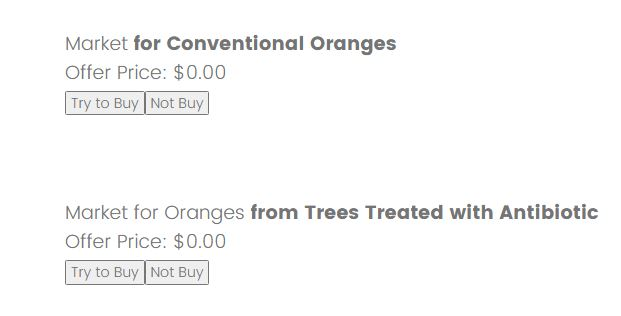
\includegraphics[width=0.8\linewidth]{GSO.JPG}
    
    \label{fig:GSO}
\end{figure}

 \vspace{0.5cm}


On the next page, you will see a video. \textbf{Please ensure your speakers or headphones are connected and the volume is set properly.} Next you will see a video that provides information about a disease Watch the video carefully in a quiet, distraction-free environment, as it is essential for the study.
\vspace{0.5cm}
Click on the video to watch it.

\href{https://www.youtube.com/watch?v=_AqMBjB0ChM}{video}
\clearpage


 \subsubsection*{Round 3}



\begin{figure}[H]
    \centering
    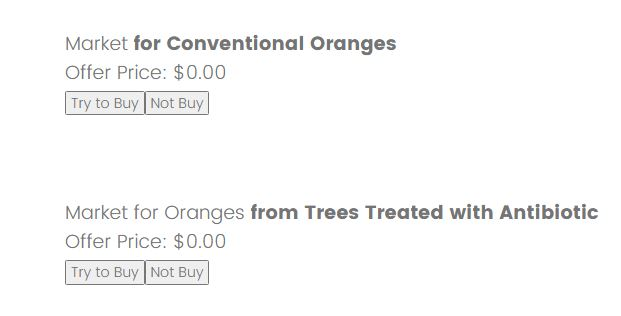
\includegraphics[width=\linewidth]{GSO.JPG}
    \caption{}
    \label{fig:Appendix_GSO_game}
\end{figure}
 

\clearpage


\subsection{GSO Real}

\subsubsection*{Instructions}

For this study you will receive a fixed fee of \$2.00 and you can earn additional compensation in cash and/or citrus products based on your decisions and chance, so please pay attention to the instructions.
 
You will complete 3 Tasks that involve real money, so please pay attention to the instructions. There is a 10\% chance that your decisions will be selected for payment. After completing the 3 tasks, the computer will draw a random number between 1 and 10. If the random number is equal to 1, you will receive the payoff as described below.
However, if the random number is between 2 and 10, your decision will not yield additional earnings, and you will receive just the \$2.00. If you are selected for payment, one of the three tasks will be randomly selected to be added to your compensation.

\textbf{Since there is a chance that your decision will end up affecting your earnings, it is in your best interest to respond carefully to each task}. If your compensation includes a food product (oranges), the product \textbf{will be shipped to your specified address *free of charge* via priority mail} as long as you provide us with a valid mailing address. You will receive more details about this procedure below.


\clearpage

\subsubsection*{Instructions (continued)}

In this study, you will complete 3 Tasks and a survey.

For each task, you will be endowed with a card with a value of \$6.00. You can use the funds in the card to purchase a bag of oranges (3.2 lbs – approximately 6-8 oranges) in two distinct markets. Any remaining funds in the card that you don’t spend on the oranges will be added to your earnings on top of your \$2.00 participation fee if you are selected for payment.

In one market, the oranges are from trees treated with antibiotics by injection to the *tree’s trunks* (not directly in the orange fruits) to prevent yield and fruit quality losses caused by a disease called citrus greening. The other market is conventional oranges, not from trees treated with antibiotics, but using a combination of pesticides and cultural practices.

You can use the funds in your card to purchase from one of the markets or both.

\textbf{ \underline{Please remember this decision is real and you may earn money or any bag of oranges.}}

\clearpage

\subsubsection*{Instructions (continued)}

 From that point, the instructions are the same as hypothetical, with a different reminder as shown below;

 Now, we will go to the main tasks.


\textbf{ \underline{Please remember this decision is real and you may earn money or any bag of oranges.}}

 \clearpage

\section{Background on citrus greening}

 The United States, which was once the world leader in citrus production, producing 50\% of the world's citrus in 1970, has experienced a decrease in its global share to 25\% in 2000, then to 5\% in 2023 \citep{munch_us_2023} . As a result of this staggering decline in domestic production, the country relies more on imports from countries such as Mexico and Chile. The recent decline in citrus production over the past 15 years in the US is mainly a result of a bacterial disease known as "Huanglongbing" (HLB) or citrus greening. This disease was first discovered in Florida in 2005, it accounts; for the infection of 80\% of citrus plants in Florida \citep{li2020citrus} and increases  production cost of farmers \citep{roka2009citrus} . This disease, caused by the bacteria "Liberibacter asiaticus", results in chlorosis of the foliage, reduction of absorption of nutrients and yield, and death of citrus trees within 3 years \citep{bove_huanglongbing_2006}. The citrus greening also affects the marketability of the citrus by distorting its size, visual feature, ripening (partial or not at all), and flavor \citep{farnsworth_potential_2024}. Orange juice made from infected citrus fruit has a higher concentration of limonin and nomilin leading to a sour taste of citrus juice \citep{paula2018active}. 

Previously, to address HLB, systematic tree removal was recommended to combat HLB. However, this approach was not sustainable for multiple reasons. First, symptomatic citrus trees could still produce some marketable fruit, making immediate tree removal financially cumbersome for farmers. Second, replacing an infected tree with a new one incurs high costs for farmers, as it takes several years before new trees begin to bear fruit.  Finally, the effect of tree removal is undermined by the external cost. If some farmers decide not to remove infected trees, the disease contributes to spreading, negating the effort of others \citep{farnsworth_potential_2024}. Recently, the administration of antibiotics through trunk injections has been investigated and found to be a promising method to control HLB \citep{li_precision_2022}. \citet{archer_trunk_2023} corroborates this discovery by showing that the administration of oxytetracyclin through injection into the trunk of orange trees results in a decrease in fruit loss before harvest, as well as an improvement in fruit output, size, and juice quality.

antibiotics administration has been applied for decades in cattle. However, according to \citet{hosain_antimicrobial_2021}, it has drawbacks on human health; it accounts for 80\% of antimicrobial resistance (AMR) in USA annually, and AMR affects 2.8 million people, causing more than 35.000 deaths \citep{cdc2019antibiotic}.  The use of antibiotics can effectively help to manage the dissemination of HLB, thus protecting citrus trees. Consequently, this can be advantageous to citrus farmers and all other stakeholders involved in the citrus industry at the state level in Florida. Antibiotics can help decrease Florida's reliance on imported citrus, thus preventing the probable extinction of citrus at the state level. This is undesirable for those who enjoy Florida citrus fruits and juice, as well as those who prefer locally sourced products. Ultimately, it can help preserve the superior taste of juice, preventing the occurrence of a bitter flavor that may arise from citrus fruits obtained from infected trees. The use of antibiotics also comes with some challenges. First, it may cause health hazards (AMR) if relevant policy is not reinforced on dosage and injection timing. Second, it may leave  residues in wastewater that could lead to soil pollution. In light of this dilemma, it directs our attention to determining how consumers will respond to the use of antibiotics in the production of citrus fruit since the success of such techniques depends on the acceptance of consumers, which also depends on the way information is communicated. Although the use of antibiotics in livestock has been extensively studied, it is unfortunate that the literature is silent about consumers’ preference for foods treated with antibiotics; hence, we propose filling this gap.

\clearpage
\section{Tables for main results}




        % Right column for the second table

            \begin{table}[htbp]
                \centering
                \caption{Descriptive Statistics by Treatment (excluding excluding MSB (R1: 14.31\%, R2, 9.6\%, R3: 3.87\%)
)}
                \label{tab:Appendix_descrip_2}
                \resizebox{1\textwidth}{!}{%
                \begin{tabular}{lccc}
                \toprule
                \textbf{Treatment}    & \textbf{N (including MSB)}       & \textbf{Mean (USD)}  & \textbf{Standard Deviation} \\
                \midrule
                GSO\_Real           & 288                        & 3.50       & 1.20                  \\
                BDM\_Real            & 313                        & 3.48       & 1.36                \\
                GSO\_Hypothetical     & 295                     & 3.63      & 1.16                   \\
                BDM\_Hypothetical      & 320                  & 3.44       & 1.30                    \\
                \midrule
                \textbf{Total}         & \textbf{1,216}              & \textbf{3.48} & \textbf{1.26}         \\
                \bottomrule
                \end{tabular}}
                \caption*{\footnotesize Note: mean and standard deviation are computed excluding MSB.}  % Footnote added here

         \end{table}
     
\clearpage
  









    \begin{table}[htbp!]
\centering
\caption{Standardized Differences Across Variables}
\label{tab:Appendix_std_diff_table}
\resizebox{\textwidth}{!}{%
\begin{tabular}{lcccccc}
\toprule

\hl& \multicolumn{3}{c}{\textbf{GSO Real vs.}} & \multicolumn{2}{c}{\textbf{BDM Real vs.}} & \textbf{GSO Hypo vs.} \\
\cmidrule(lr){2-4} \cmidrule(lr){5-6} \cmidrule(lr){7-7}
\textbf{Variable}        & \textbf{BDM Real} & \textbf{GSO Hypo} & \textbf{BDM Hypo} & \textbf{GSO Hypo} & \textbf{BDM Hypo} & \textbf{BDM Hypo} \\
\midrule

Hispanic        & 0.0963        & 0.0184        & 0.0784        & 0.0778        & 0.0179        & 0.0599 \\
Income category & 0.1668        & 0.0547        & 0.1489        & 0.1557        & 0.0303        & 0.1306 \\
Region  & 0.1132        & 0.1649        & 0.1624        & 0.0900        & 0.0701        & 0.0623 \\
Gender  & 0.0788        & 0.0074        & 0.0432        & 0.0713        & 0.0356        & 0.0357 \\
Education      & 0.1812        & 0.1340        & 0.1308        & 0.0469        & 0.0501        & 0.0032 \\
Children        & 0.0701        & 0.0253        & 0.0795        & 0.0448        & 0.0094        & 0.0542 \\
Marital status  & 0.0342        & 0.0391        & 0.0239        & 0.0733        & 0.0103        & 0.0630 \\
Age     & -0.0053       & 0.0819        & -0.0541       & 0.0836        & -0.0467       & -0.1327 \\


\bottomrule
\end{tabular}}
\begin{tablenotes}
\item Notes: GSO stands for the Game Structure Obvious mechanism treatment; BDM stands for the Becker-DeGroot-Marschak mechanism treatment; Real and Hypo stand for the real and hypothetical incentives treatments, respectively.
\end{tablenotes}
\end{table}
    %   \vspace{0.2em} % Add some vertical spacing before the note
    
    % \footnotesize % Use smaller font size for the note
    % \textbf{Note:} 1:Randomization achieved once value is lower than 0.25.
 
\clearpage










 \begin{table}[H]
        \centering
        \caption{Comparison of Willingness to Pay by Instruction Comprehension Scores (aggregate) }
        \label{tab:MSB_interval_regression_Score_overall}
        \resizebox{0.7\textwidth}{!}{% Scale table to fit the column width
  \begin{tabular}{l*{2}{cc}}
\hline\hline
            &\multicolumn{2}{c}{(1)}           &\multicolumn{2}{c}{(2)}           \\
            &\multicolumn{2}{c}{WTP (GSO)}    &\multicolumn{2}{c}{WTP (BDM)}    \\
\hline
Constant    &       3.136\sym{***}&     (0.169)&       2.937\sym{***}&     (0.096)\\
Hypothetical&       0.026         &     (0.145)&       0.084         &     (0.075)\\
test\_score  &       0.039\sym{**} &     (0.017)&       0.027\sym{***}&     (0.009)\\
Hypothetical$\times$test\_score&       0.036         &     (0.023)&      -0.021\sym{*}  &     (0.012)\\
Round2      &       0.048         &     (0.049)&       0.064\sym{*}  &     (0.034)\\
Round3      &       0.096\sym{*}  &     (0.054)&       0.116\sym{***}&     (0.035)\\
Risk preferences&      -0.069\sym{***}&     (0.024)&      -0.165\sym{***}&     (0.016)\\
MSB      &       1.079\sym{***}&     (0.102)&                     &            \\
White&      -0.077         &     (0.052)&      -0.037         &     (0.032)\\
Middle Income&      -0.047         &     (0.058)&      -0.063\sym{*}  &     (0.034)\\
High Income&       0.413\sym{***}&     (0.101)&      -0.153\sym{***}&     (0.059)\\
Midwest   &      -0.152\sym{**} &     (0.076)&      -0.258\sym{***}&     (0.049)\\
South    &      -0.091         &     (0.065)&      -0.125\sym{***}&     (0.042)\\
West    &      -0.184\sym{**} &     (0.077)&      -0.147\sym{***}&     (0.049)\\
Female    &      -0.085\sym{*}  &     (0.048)&       0.154\sym{***}&     (0.028)\\
Bachelor&      -0.240\sym{***}&     (0.052)&       0.073\sym{**} &     (0.032)\\
No Children  &       0.150\sym{***}&     (0.058)&      -0.111\sym{***}&     (0.035)\\
Married&      -0.227\sym{***}&     (0.060)&       0.026         &     (0.031)\\
Age         &       0.009\sym{***}&     (0.002)&       0.010\sym{***}&     (0.001)\\
$\sigma_u$     &       1.118\sym{***}&     (0.025)&       1.006\sym{***}&     (0.015)\\
$\sigma_e$    &       0.812\sym{***}&     (0.030)&       0.841\sym{***}&     (0.015)\\

\hline
\(n\) (observations)       &        3408         &            &        3702         &            \\
\(N\) (subjects)       &        568         &            &        617         &            \\
\hline\hline
\multicolumn{5}{l}{\footnotesize Standard errors in parentheses. * p$<$0.1, ** p$<$0.05 *** p$<$0.01}\\
\end{tabular}
}





\begin{tablenotes}
            \footnotesize
            \item Standard errors in parentheses. * p$<$0.1, ** p$<$0.05, *** p$<$0.01.
            \item \textit{Note:} $\sigma_u$ and $\sigma_e$ denote the standard deviations of the random intercept and residual error, respectively.\\
            $\times$: interaction\\
            Real incentive represents the baseline.\\
        \end{tablenotes}
\end{table}
\clearpage




     
 \begin{table}[H]
        \centering
        \caption{Comparison of Willingness to Pay by Instruction Comprehension Scores (Top and Bottom Quartiles) for GSO}
        \label{tab:MSB_interval_regression_Scorehigh_low}
        \resizebox{0.7\textwidth}{!}{% Scale table to fit the column width
      \begin{tabular}{l*{1}{cc}}
\hline\hline
            &\multicolumn{2}{c}{(1)}           \\
            &\multicolumn{2}{c}{WTP}    \\
\hline
Constant    &       3.579\sym{***}&     (0.155)\\
Hypothetical&       0.160\sym{**} &     (0.071)\\
Top 25\%     &      -0.255\sym{**} &     (0.105)\\
Top25\%$\times$Hypothetical&       1.002\sym{***}&     (0.149)\\
AntibioticsOranges&      -0.190\sym{*}  &     (0.099)\\
Round2     &      -0.065         &     (0.090)\\
Round3     &      -0.181\sym{*}  &     (0.093)\\
AntibioticsOranges$\times$Round2&       0.099         &     (0.135)\\
AntibioticsOranges$\times$Round3&       0.321\sym{**} &     (0.137)\\
Risk preferences&      -0.036         &     (0.030)\\
White       &       0.050         &     (0.073)\\
Middle Income&      -0.095         &     (0.074)\\
High Income &       0.473\sym{***}&     (0.120)\\
Midwest     &       0.041         &     (0.103)\\
South       &       0.100         &     (0.086)\\
West        &      -0.041         &     (0.101)\\
Female      &      -0.139\sym{**} &     (0.063)\\
Bachelor    &      -0.251\sym{***}&     (0.071)\\
No Children &       0.160\sym{**} &     (0.073)\\
Married     &      -0.368\sym{***}&     (0.073)\\
Age         &       0.007\sym{***}&     (0.002)\\
$\sigma_u$     &       1.099\sym{***}&     (0.032)\\
$\sigma_e$     &       0.852\sym{***}&     (0.040)\\
\hline
\(n\) (observations)       &        2118         &            \\
\(N\) (subjects)       &        353         &            \\
\hline\hline
\end{tabular}
}



\begin{tablenotes}
            \footnotesize
            \item Standard errors in parentheses. * p$<$0.1, ** p$<$0.05, *** p$<$0.01.
            \item \textit{Note:} $\sigma_u$ and $\sigma_e$ denote the standard deviations of the random intercept and residual error, respectively.\\
            $\times$: interaction\\
        \end{tablenotes}
\end{table}
\clearpage

 \begin{table}[H]
        \centering
        \caption{Comparison of Willingness to Pay by Instruction Comprehension Scores (Top and Bottom Quartiles) for BDM}
        \label{tab:MSB_interval_regression_BDM_Scorehigh_low}
        \resizebox{0.7\textwidth}{!}{% Scale table to fit the column width
      \begin{tabular}{l*{1}{cc}}
\hline\hline
            &\multicolumn{2}{c}{WTP}    \\
\hline
Constant    &       3.011\sym{***}&     (0.090)\\
Hypothetical&      -0.060         &     (0.042)\\
Top 25\%     &       0.087         &     (0.058)\\
Top25\%$\times$Hypothetical&       0.137\sym{*}  &     (0.077)\\
AntibioticsOranges&      -0.032         &     (0.056)\\
Round2     &       0.056         &     (0.057)\\
Round3     &      -0.057         &     (0.057)\\
AntibioticsOranges$\times$Round2&       0.072         &     (0.077)\\
AntibioticsOranges$\times$Round3&       0.377\sym{***}&     (0.079)\\
Risk preferences&      -0.189\sym{***}&     (0.017)\\
White       &      -0.043         &     (0.036)\\
Middle Income&      -0.206\sym{***}&     (0.039)\\
High Income &      -0.200\sym{***}&     (0.069)\\
Midwest     &      -0.111\sym{**} &     (0.053)\\
South       &      -0.006         &     (0.050)\\
West        &       0.044         &     (0.056)\\
Female      &       0.064\sym{*}  &     (0.033)\\
Bachelor    &       0.157\sym{***}&     (0.042)\\
No Children &      -0.166\sym{***}&     (0.036)\\
Married     &       0.096\sym{***}&     (0.036)\\
Age         &       0.011\sym{***}&     (0.001)\\
$\sigma_u$      &       0.973\sym{***}&     (0.016)\\
$\sigma_e$      &       0.815\sym{***}&     (0.018)\\
\hline
\(n\) (observations)      &        2544         &            \\
\(N\) (subjects)      &        424         &            \\
\hline\hline
\multicolumn{3}{l}{\footnotesize Standard errors in parentheses.	*	p$<$0.1,	**	p$<$0.05	***	p$<$0.01}\\
\end{tabular}
}

\begin{tablenotes}
            \footnotesize
          
            \item \textit{Note:} $\sigma_u$ and $\sigma_e$ denote the standard deviations of the random intercept and residual error, respectively.\\
            $\times$: interaction\\
        \end{tablenotes}
\end{table}


\clearpage





\begin{table}[H]
        \centering
        \caption{Comparison of Willingness to Pay by multiple switching behavior (MSB)}
        \label{tab:MSB_interval_regression_MSB}
        \resizebox{0.7\textwidth}{!}{% Scale table to fit the column width
      \begin{tabular}{l*{1}{cc}}
\hline\hline
            &\multicolumn{2}{c}{WTP}    \\
\hline
Constant    &       3.367\sym{***}&     (0.124)\\
Hypothetical&       0.232\sym{***}&     (0.056)\\
MSB      &       1.018\sym{***}&     (0.166)\\
Hypothetical$\times$MSB&       0.107         &     (0.211)\\
Round2      &       0.047         &     (0.049)\\
Round3      &       0.096\sym{*}  &     (0.054)\\
Risk preferences&      -0.070\sym{***}&     (0.023)\\
White&      -0.080         &     (0.052)\\
Midlle Income &      -0.051         &     (0.057)\\
High Income&       0.388\sym{***}&     (0.101)\\
Midwest    &      -0.120         &     (0.076)\\
South    &      -0.061         &     (0.064)\\
West    &      -0.177\sym{**} &     (0.077)\\
Female    &      -0.080\sym{*}  &     (0.048)\\
Bachelor&      -0.254\sym{***}&     (0.052)\\
No children  &       0.147\sym{**} &     (0.058)\\
Married&      -0.233\sym{***}&     (0.060)\\
Age         &       0.009\sym{***}&     (0.002)\\
$\sigma_u$     &       1.126\sym{***}&     (0.025)\\
$\sigma_e$     &       0.812\sym{***}&     (0.030)\\

\hline
\(n\) (observations)       &        3408         &            \\
\(n\) (subjects)       &        568         &            \\
\hline\hline
\multicolumn{3}{l}{\footnotesize Standard errors in parentheses.	*	p$<$0.1,	**	p$<$0.05	***	p$<$0.01}\\
\end{tabular}
}

\begin{tablenotes}
            \footnotesize
          
            \item \textit{Note:} $\sigma_u$ and $\sigma_e$ denote the standard deviations of the random intercept and residual error, respectively.\\
            $\times$: interaction\\
        \end{tablenotes}
\end{table}

\clearpage






\begin{table}[H]
    \centering
    \caption{Time spent across elicitation tasks}
    \label{tab:my_label}
\resizebox{\textwidth}{!}{%
\begin{tabular}{lcccc}
\toprule
\textbf{Statistic} & \multicolumn{2}{c}{\textbf{GSO (no MSB)}} & \multicolumn{2}{c}{\textbf{BDM}} \\
\cmidrule(lr){2-3} \cmidrule(lr){4-5}
& Hypothetical & Real & Hypothetical & Real \\
\midrule
n (observations)         & 1,770 & 1,728 & 1,920 & 1,878 \\
Mean                       &  10.5 & 9.5 & 4{,}107.2 & 4{,}8165 \\
Standard Error             & 0.20 & 0.20 & 296.37 & 484.66 \\
Standard Deviation         & 8.6  & 8.45 & 12{,}986.42 & 21{,}003.45 \\

Difference in Means        & \multicolumn{2}{c}{0.998} & \multicolumn{2}{c}{-709.05} \\
Std. Error of Difference   & \multicolumn{2}{c}{ 0.288} & \multicolumn{2}{c}{569.3} \\
$p$-value (two-sided)      & \multicolumn{2}{c}{ 0.0006} & \multicolumn{2}{c}{0.2048} \\

\bottomrule
\end{tabular}%
}
\end{table}

\clearpage

\begin{table}[H]
        \centering
        \caption{Comparison of Willingness to Pay by Round for GSO}
        \label{tab:interval_regression_RounbyRound}
        \resizebox{0.7\textwidth}{!}{% Scale table to fit the column width
     \begin{tabular}{l*{2}{cc}}
\hline\hline
            &\multicolumn{2}{c}{(1)}           &\multicolumn{2}{c}{(2)}           \\
            &\multicolumn{2}{c}{WTP (GSO)}    &\multicolumn{2}{c}{WTP (BDM)}    \\
\hline
Constant    &       3.329\sym{***}&     (0.126)&       3.114\sym{***}&     (0.075)\\
Hypothetical&       0.308\sym{***}&     (0.078)&      -0.053         &     (0.052)\\
Round2      &       0.103         &     (0.072)&       0.079         &     (0.050)\\
Round3      &       0.142\sym{*}  &     (0.073)&       0.079         &     (0.050)\\
Hypothetical$\times$Round2&      -0.109         &     (0.100)&      -0.029         &     (0.070)\\
Hypothetical$\times$Round3&      -0.089         &     (0.107)&       0.074         &     (0.071)\\
Risk preferences&      -0.069\sym{***}&     (0.023)&      -0.165\sym{***}&     (0.016)\\
MSB     &       1.080\sym{***}&     (0.102)&                     &            \\
White&      -0.080         &     (0.052)&      -0.044         &     (0.031)\\
Middle Income&      -0.050         &     (0.057)&      -0.062\sym{*}  &     (0.034)\\
High Income&       0.386\sym{***}&     (0.100)&      -0.150\sym{**} &     (0.059)\\
Midwest   &      -0.119         &     (0.076)&      -0.263\sym{***}&     (0.049)\\
South    &      -0.062         &     (0.064)&      -0.130\sym{***}&     (0.042)\\
West    &      -0.178\sym{**} &     (0.077)&      -0.155\sym{***}&     (0.049)\\
Female    &      -0.079\sym{*}  &     (0.048)&       0.156\sym{***}&     (0.028)\\
Bachelor&      -0.253\sym{***}&     (0.052)&       0.067\sym{**} &     (0.032)\\
No Children  &       0.149\sym{**} &     (0.058)&      -0.107\sym{***}&     (0.035)\\
Married&      -0.234\sym{***}&     (0.060)&       0.025         &     (0.031)\\
Age         &       0.009\sym{***}&     (0.002)&       0.010\sym{***}&     (0.001)\\
MSB      &                     &            &       0.000         &     (0.000)\\
$\sigma_u $    &       1.126\sym{***}&     (0.025)&       1.007\sym{***}&     (0.015)\\
$\sigma_e $    &       0.812\sym{***}&     (0.030)&       0.840\sym{***}&     (0.015)\\
\hline
\(n\) (observations)      &        3408         &            &        3702         &            \\
\(N\) (subjects)      &        568         &            &        617         &            \\
\hline\hline
\multicolumn{5}{l}{\footnotesize Standard errors in parentheses. * p$<$0.1, ** p$<$0.05 *** p$<$0.01}\\
\end{tabular}
}



\begin{tablenotes}
            \footnotesize
          
            \item \textit{Note:} $\sigma_u$ and $\sigma_e$ denote the standard deviations of the random intercept and residual error, respectively.\\
            $\times$: interaction\\
        \end{tablenotes}
\end{table}





\clearpage






\clearpage


    \begin{table}[htbp!]
        \centering
        \caption{Two-Sample Test of Proportions (complexity above median)}
        \label{tab:Appendix_proportion_test}
        \resizebox{0.9\textwidth}{!}{% Scale table to fit the column width
        \begin{tabular}{lcccccc}
\hline\hline
\textbf{Group} & \textbf{Obs} & \textbf{Mean} & \textbf{Std. Err.} & \textbf{z} & \textbf{$P>|z|$} & \textbf{95\% Conf. Interval (Lower)}  \\
\hline
BDM            & 3,798        & 0.4186414     & 0.008           &            &                 & [0.40, 0.43]                             \\
GSO            & 2,376        & 0.36     & 0.008          &            &                 & [0.35, 0.38]                               \\
\hline
\textbf{Diff}  &              & 0.05    & 0.011          & 4.35     & 0.000           & [0.027, 0.072]                             \\
\hline\hline
        \end{tabular}
        }
    \end{table}


\clearpage

\begin{table}[htbp!]
    \centering
    \caption{Two-Sample Test of Proportions by Complexity above median (Group MSB vs. Non-MSB)}
    \label{tab:Appendix_proportion_test_groupMSB_vs_Non-MSB}
    \resizebox{0.9\textwidth}{!}{%
    \begin{tabular}{lcccccc}
\hline\hline
\textbf{Group} & \textbf{Obs} & \textbf{Mean} & \textbf{Std. Err.} & \textbf{z} & \textbf{$P>|z|$} & \textbf{95\% Conf. Interval (Lower)} \\
\hline
Non-MSB             & 6,174        & 0.3732        & 0.0062              &            &                  & [0.3611, 0.3852]                    \\
MSB              & 1,122        & 0.5134        & 0.0149              &            &                  & [0.4841, 0.5426]                    \\
\hline
\textbf{Diff}  &              & -0.1402       & 0.0161              & -8.84      & 0.000            & [-0.1718, -0.1086]                  \\
\hline\hline
    \end{tabular}
    }
\end{table}

\clearpage





\begin{table}[htbp!]
    \centering
    \caption{Game form recognition}
    \label{tab:Appendix_gameform}
    \resizebox{0.9\textwidth}{!}{%
    \begin{tabular}{lcccc}
    \toprule
    \textbf{Variable} & \textbf{Group} & \textbf{Mean} & \textbf{Std. Dev.} & \textbf{t-stat (p-value)} \\
    \midrule
    \multirow{\text{Complexity score}} 
      & BDM & 2.33 & 1.06 & \multirow{\ensuremath{(p < 0.01)}} \\
      & GSO & 2.19 & 1.06 & \\
    \midrule
    \multirow{\text{Choice certainty}} 
      & BDM & 3.66 & 1.01 & \multirow{\ensuremath{\ (p < 0.01)}} \\
      & GSO & 3.74 & 0.99 & \\
    \bottomrule
    \end{tabular}%
    }
\end{table}


\clearpage
%%%%%%%%%%%%%%%%%%%%%%%%%%%%%%%%%%%%%%%%%%%%%%%%%%%%%%%%%%%%%%%%%%%%%%%%%%%%%%%%%%%%%%%%%%%%%%%%%%%%%%%%%%%%%%%%%%%%%%%%%%%%%%a%%%%%%
\section{Appendix sections including multiple switchers}




 \begin{table}[H]
                \centering
                \caption{Interval Model of Consumer WTP for Oranges (Baseline: BDM Real)}
                \label{tab:MSB_interval_regression_multiple_comaparisons}
                \resizebox{0.85\textwidth}{!}{% Scale table to fit the column width
             \begin{tabular}{l*{3}{cc}}
\hline\hline
            &\multicolumn{2}{c}{(1)}           &\multicolumn{2}{c}{(2)}           &\multicolumn{2}{c}{(3)}           \\
            &\multicolumn{2}{c}{WTP     (full sample)}    &\multicolumn{2}{c}{WTP (exclude MSB)}    &\multicolumn{2}{c}{WTP (only MSB)}    \\
\hline
Constant    &       3.187\sym{***}&     (0.066)&       3.197\sym{***}&     (0.068)&       3.169\sym{***}&     (0.067)\\
GSO         &       0.014         &     (0.040)&       0.015         &     (0.041)&       1.230\sym{***}&     (0.071)\\
Hypothetical&      -0.037         &     (0.033)&      -0.037         &     (0.036)&      -0.038         &     (0.032)\\
GSO$\times$Hypothetical&       0.277\sym{***}&     (0.057)&       0.271\sym{***}&     (0.063)&       0.144         &     (0.094)\\
Round2      &       0.060\sym{**} &     (0.029)&       0.052\sym{*}  &     (0.028)&       0.069\sym{**} &     (0.033)\\
Round3      &       0.111\sym{***}&     (0.029)&       0.108\sym{***}&     (0.030)&       0.118\sym{***}&     (0.035)\\
MSB      &       1.088\sym{***}&     (0.090)&                     &            &                     &            \\
Risk preferences&      -0.120\sym{***}&     (0.014)&      -0.118\sym{***}&     (0.014)&      -0.157\sym{***}&     (0.016)\\
White&      -0.058\sym{**} &     (0.029)&      -0.062\sym{**} &     (0.029)&      -0.027         &     (0.029)\\
Middle Income&      -0.045         &     (0.031)&      -0.055\sym{*}  &     (0.033)&      -0.018         &     (0.030)\\
High income&       0.065         &     (0.048)&       0.067         &     (0.053)&      -0.109\sym{**} &     (0.054)\\
Midwest    &      -0.186\sym{***}&     (0.042)&      -0.197\sym{***}&     (0.044)&      -0.235\sym{***}&     (0.046)\\
South    &      -0.094\sym{**} &     (0.037)&      -0.082\sym{**} &     (0.039)&      -0.158\sym{***}&     (0.040)\\
West   &      -0.158\sym{***}&     (0.040)&      -0.151\sym{***}&     (0.044)&      -0.180\sym{***}&     (0.045)\\
female    &       0.061\sym{**} &     (0.025)&       0.049\sym{*}  &     (0.027)&       0.153\sym{***}&     (0.028)\\
Bachelor&      -0.084\sym{***}&     (0.030)&      -0.098\sym{***}&     (0.033)&       0.066\sym{**} &     (0.031)\\
No children  &       0.004         &     (0.030)&      -0.003         &     (0.033)&      -0.062\sym{*}  &     (0.032)\\
Married&      -0.086\sym{***}&     (0.031)&      -0.103\sym{***}&     (0.032)&       0.021         &     (0.029)\\
Age         &       0.010\sym{***}&     (0.001)&       0.010\sym{***}&     (0.001)&       0.008\sym{***}&     (0.001)\\
$\sigma_u$     &       1.064\sym{***}&     (0.012)&       1.087\sym{***}&     (0.013)&       0.956\sym{***}&     (0.013)\\
$\sigma\e $    &       0.835\sym{***}&     (0.014)&       0.834\sym{***}&     (0.014)&       0.834\sym{***}&     (0.015)\\

\hline
\(n\) (observations)       &        7110         &            &        6036         &            &        4776         &            \\
\hline\hline
\multicolumn{7}{l}{\footnotesize Standard errors in parentheses. * p$<$0.1, ** p$<$0.05 *** p$<$0.01}\\
\end{tabular}
}


\begin{tablenotes}
            \footnotesize
            \item Standard errors in parentheses. * p$<$0.1, ** p$<$0.05, *** p$<$0.01.
            \item \textit{Note:} $\sigma_u$ and $\sigma_e$ denote the standard deviations of the random intercept and residual error, respectively.\\
            $\times$: interaction\\
        \end{tablenotes}
            \end{table}


\clearpage







            \begin{table}[htbp!]
                \centering
                \caption{The table below diplays column 1 is for GSO and column 2 is for BDM (Baseline: Real) }
                \label{tab:MSB_Appendix_interval_BDM_GSO}
                % \resizebox{\textwidth}{!}{% Scale table to fit the column width
      \begin{tabular}{l*{2}{cc}}
\hline\hline
            &\multicolumn{2}{c}{(1)}           &\multicolumn{2}{c}{(2)}           \\
            &\multicolumn{2}{c}{WTP (GSO)}      &\multicolumn{2}{c}{WTP (BDM)}    \\
\hline

Constant    &       3.365\sym{***}&     (0.185)&       3.110\sym{***}&     (0.119)\\
Hypothetical&       0.240\sym{***}&     (0.085)&      -0.043         &     (0.043)\\
AntibioticsOranges&      -0.068\sym{*}  &     (0.039)&      -0.029         &     (0.073)\\
Round2     &      -0.009         &     (0.039)&       0.036         &     (0.070)\\
Round3     &      -0.028         &     (0.042)&      -0.059         &     (0.071)\\
AntibioticsOranges$\times$Round2&       0.051         &     (0.054)&       0.056         &     (0.104)\\
AntibioticsOranges$\times$Round3&       0.119\sym{**} &     (0.056)&       0.350\sym{***}&     (0.106)\\
Risk preferences&      -0.115\sym{**} &     (0.058)&      -0.162\sym{***}&     (0.024)\\
White       &      -0.045         &     (0.102)&      -0.041         &     (0.049)\\
Middle Income&      -0.158         &     (0.103)&      -0.066         &     (0.050)\\
High Income &       0.300         &     (0.189)&      -0.151         &     (0.092)\\
Midwest     &      -0.007         &     (0.150)&      -0.262\sym{***}&     (0.072)\\
South       &      -0.036         &     (0.121)&      -0.122\sym{*}  &     (0.065)\\
West        &      -0.064         &     (0.169)&      -0.154\sym{**} &     (0.072)\\
Female      &      -0.020         &     (0.088)&       0.156\sym{***}&     (0.044)\\
Bachelor    &      -0.227\sym{**} &     (0.106)&       0.065         &     (0.049)\\
No Children &       0.040         &     (0.105)&      -0.106\sym{**} &     (0.051)\\
Married     &      -0.292\sym{**} &     (0.115)&       0.031         &     (0.049)\\
Age         &       0.009\sym{***}&     (0.003)&       0.010\sym{***}&     (0.001)\\
$\sigma_u$    &       1.358\sym{***}&     (0.074)&                     &            \\
$\sigma_u$    &       0.470\sym{***}&     (0.044)&                     &            \\
\hline
\(n\) (observations)       &        3408         &            &        3702         &            \\
\hline\hline
\multicolumn{5}{l}{\footnotesize Standard errors in parentheses. * p$<$0.1, ** p$<$0.05 *** p$<$0.01}\\
\end{tabular}
% }


\begin{tablenotes}
            \footnotesize
            \item Standard errors in parentheses. * p$<$0.1, ** p$<$0.05, *** p$<$0.01.
            \item \textit{Note:} $\sigma_u$ and $\sigma_e$ denote the standard deviations of the random intercept and residual error, respectively.\\
            $\times$: interaction\\
        \end{tablenotes}
            \end{table}
      

\clearpage










\end{document}